
\chapter{Execution Evidence}

\section{Test Cases}

\subsection{Factorial}

\begin{verbatim}
#| Iterative factorial implementation |#
proc fact_iter(n int) -> int 
    var acc int;
{
    loop acc <- 1; n > 0; n <- n - 1 {
        acc <- n * acc;
    }
    
    return acc;
}

#| Recursive factorial implementation |#
proc fact_rec(n int) -> int {
    if n <= 0 {
        return 1;
    } else {
        return n * fact_rec(n - 1);
    }
}
\end{verbatim}

\newpage

\begin{verbatim}
#| Main procedure |#
proc main() 
    var f1, f2, i int;
{
    loop {
        print("=== Factorial ===");

        i <- read("Type value calculate factorial");

        f1 <- fact_iter(i);
        f2 <- fact_rec(i);

        print("Iterative answer", f1);
        print("Recursive answer", f2);
    }
}
\end{verbatim}

\begin{figure}[h]
    \centering
    \caption{Generated IR code}
    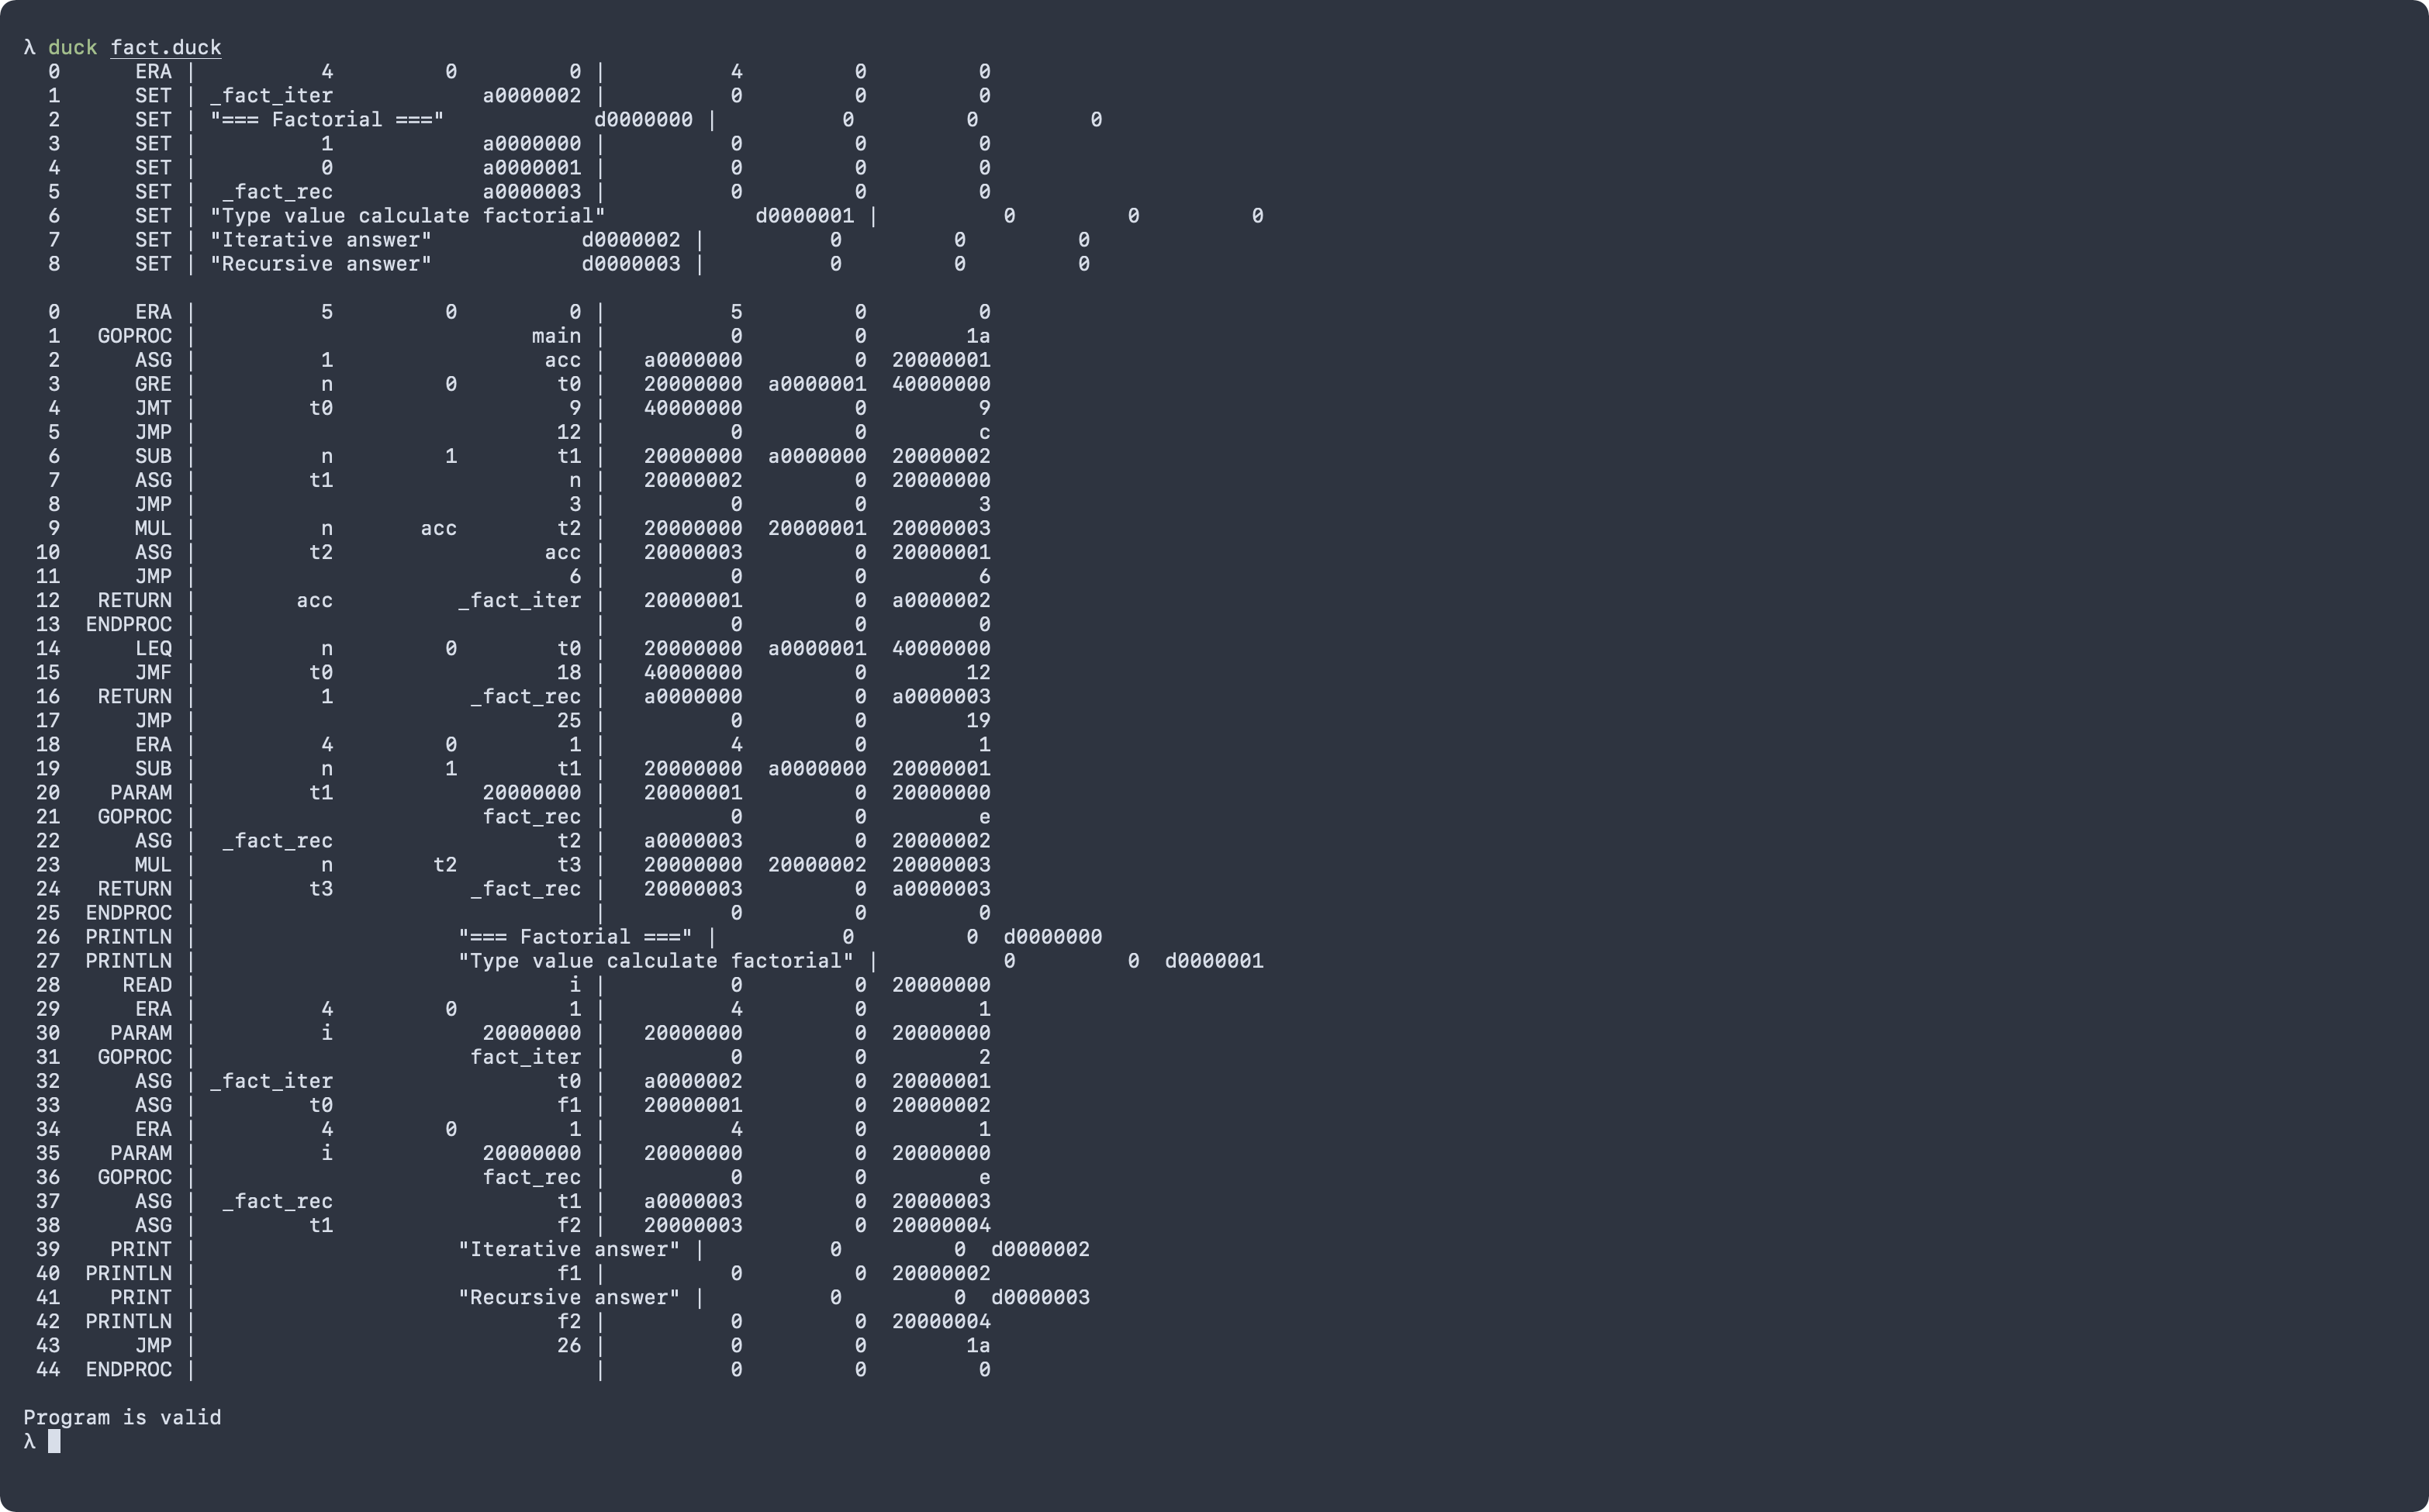
\includegraphics[width=\textwidth]{evidences/fact_ir}
\end{figure}

\newpage

\begin{figure}[h]
    \centering
    \caption{Program output}
    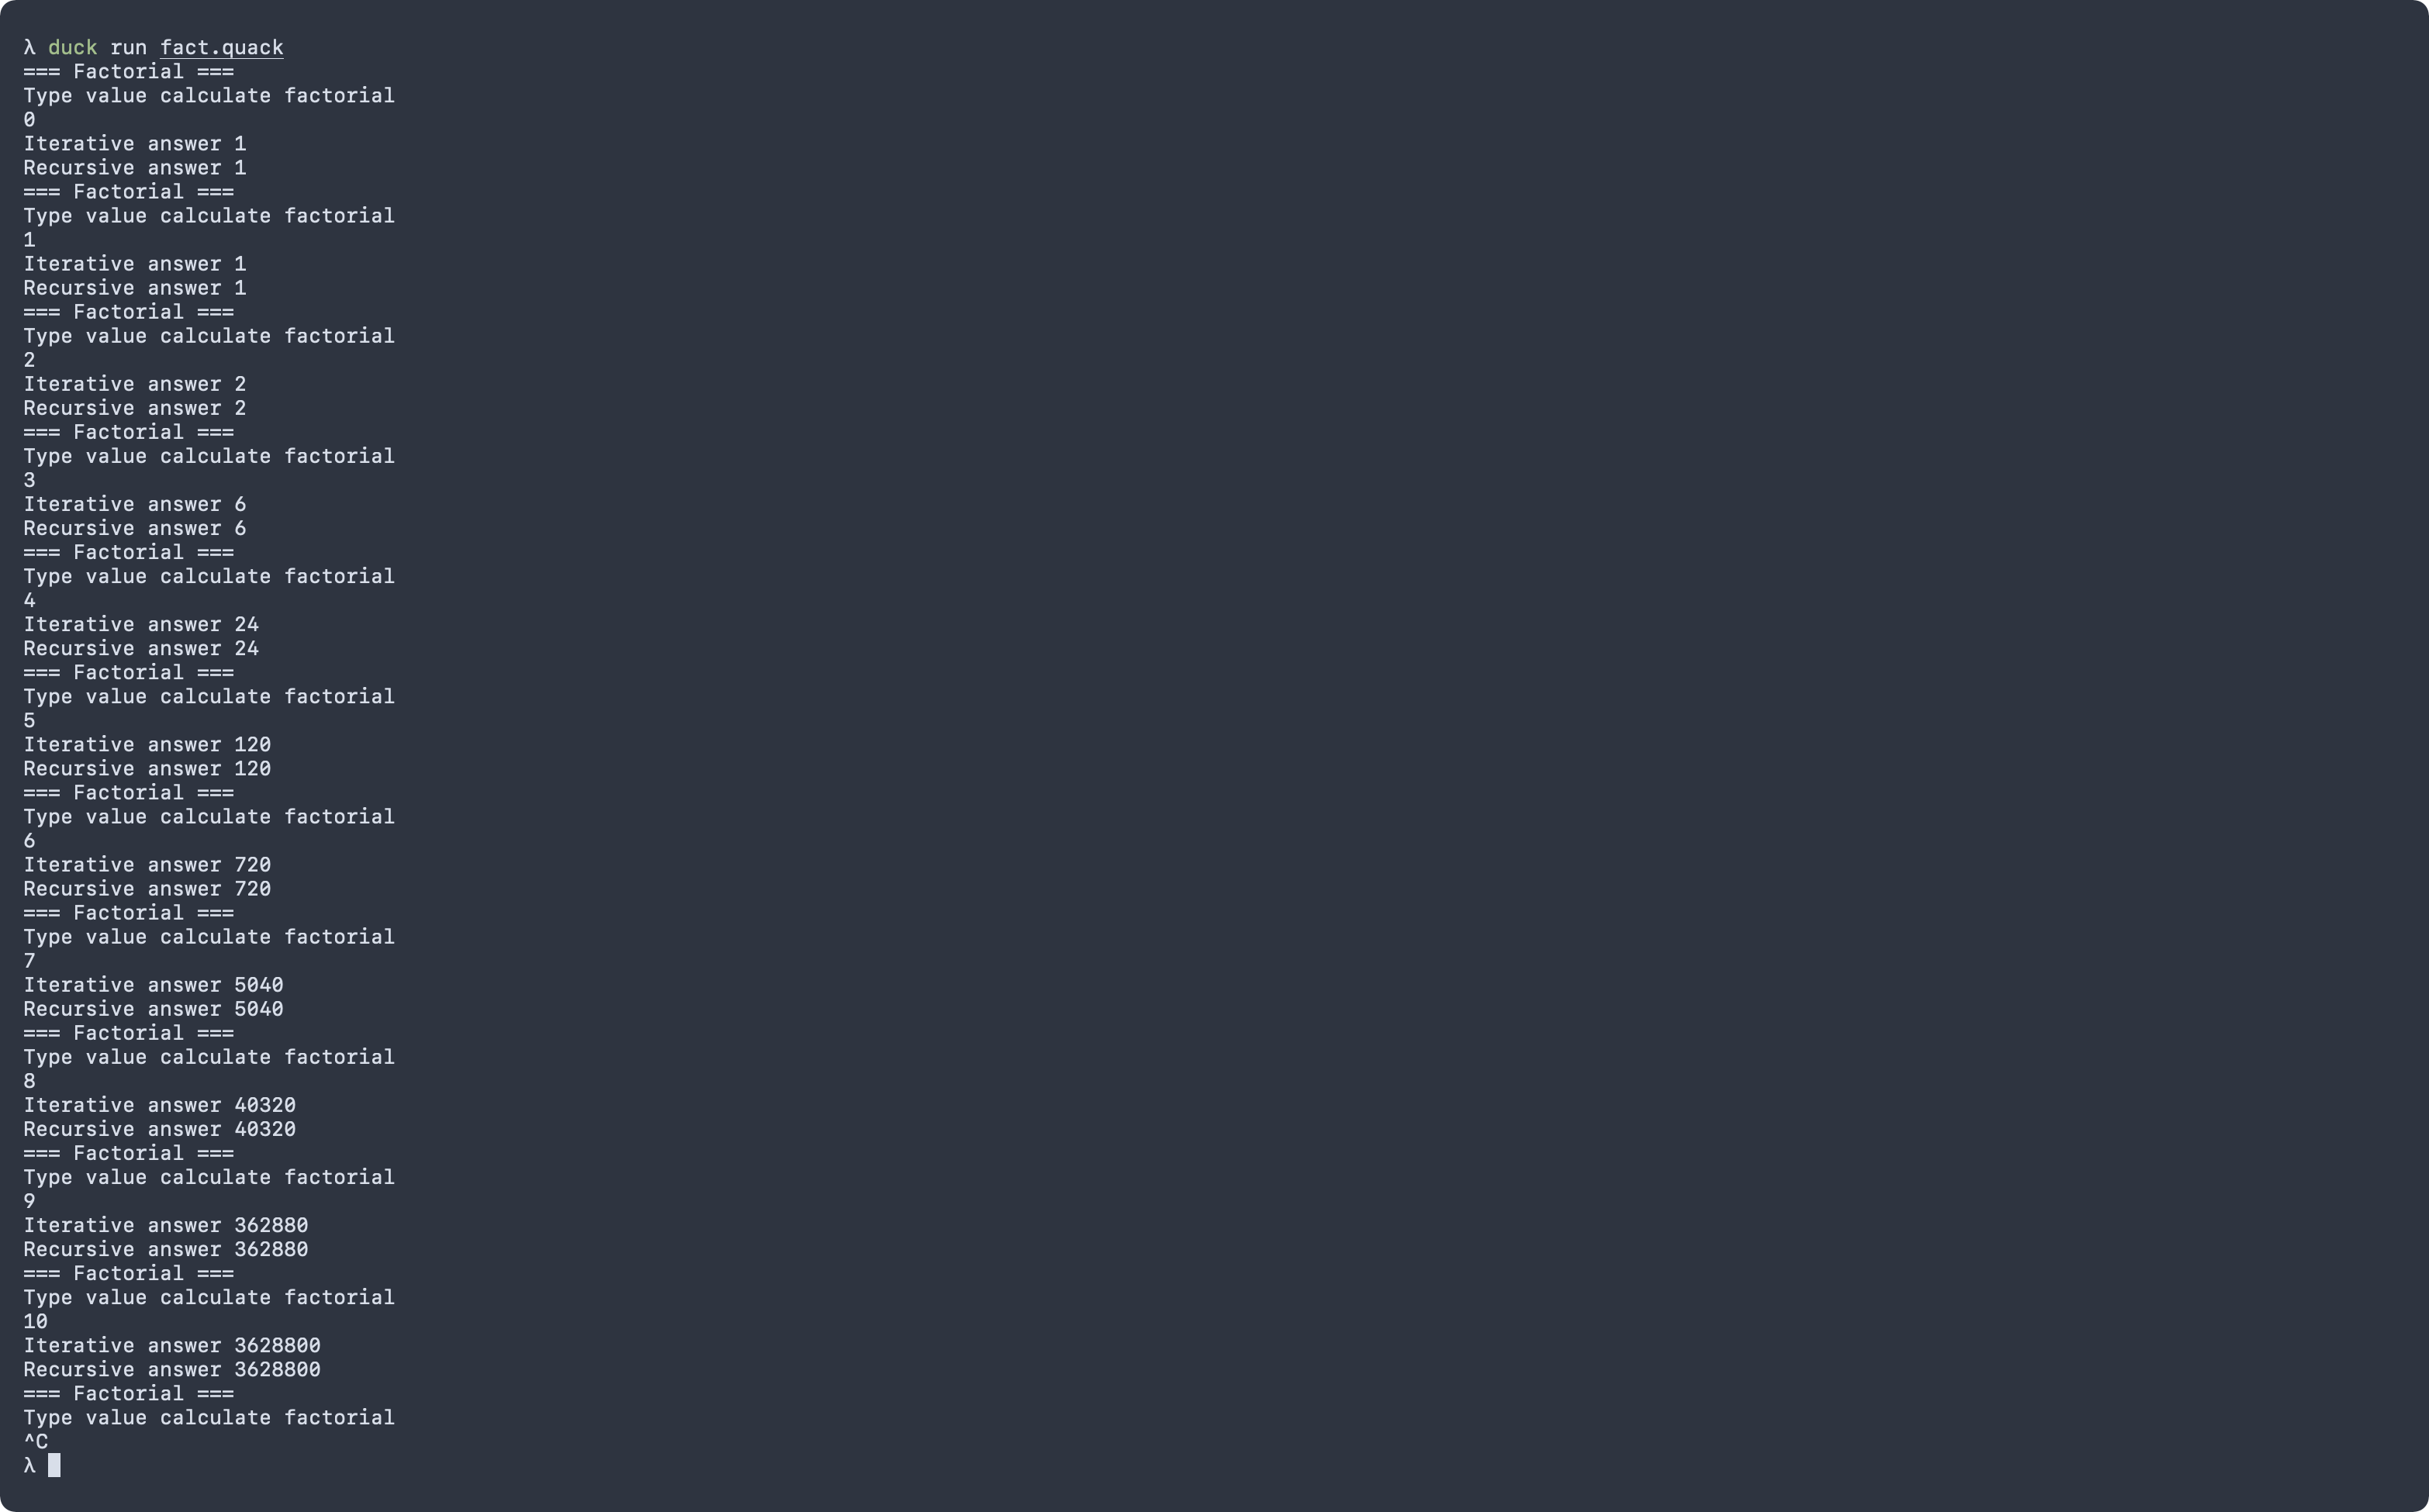
\includegraphics[width=\textwidth]{evidences/fact_output}
\end{figure}

\subsection{Fibonacci}

\begin{verbatim}
#| Iterative fibbonaci implementation |#
proc fib_iter(n int) -> int 
    var f0, f1, tmp int;
{
    f0 <- 0;
    f1 <- 1;

    loop ; n > 0; n <- n - 1 {
        tmp <- f1;
        f1 <- f0 + f1;
        f0 <- tmp;
    }
    
    return f0;
}

\end{verbatim}

\newpage

\begin{verbatim}
#| Recursive fibbonaci implementation |#
proc fib_rec(n int) -> int {
    if n <= 0 {
        return 0;
    } else if n = 1 {
        return 1;
    } else {
        return fib_rec(n - 1) + fib_rec(n - 2);
    }
}

#| Main procedure |#
proc main() 
    var f1, f2, i int;
{
    loop {
        print("=== Fibonacci ===");

        i <- read("Type value of the nth fibonacci to calculate");

        f1 <- fib_iter(i);
        f2 <- fib_rec(i);

        print("Iterative answer", f1);
        print("Recursive answer", f2);
    }
}
\end{verbatim}

\begin{figure}[H]
    \centering
    \caption{Generated IR code}
    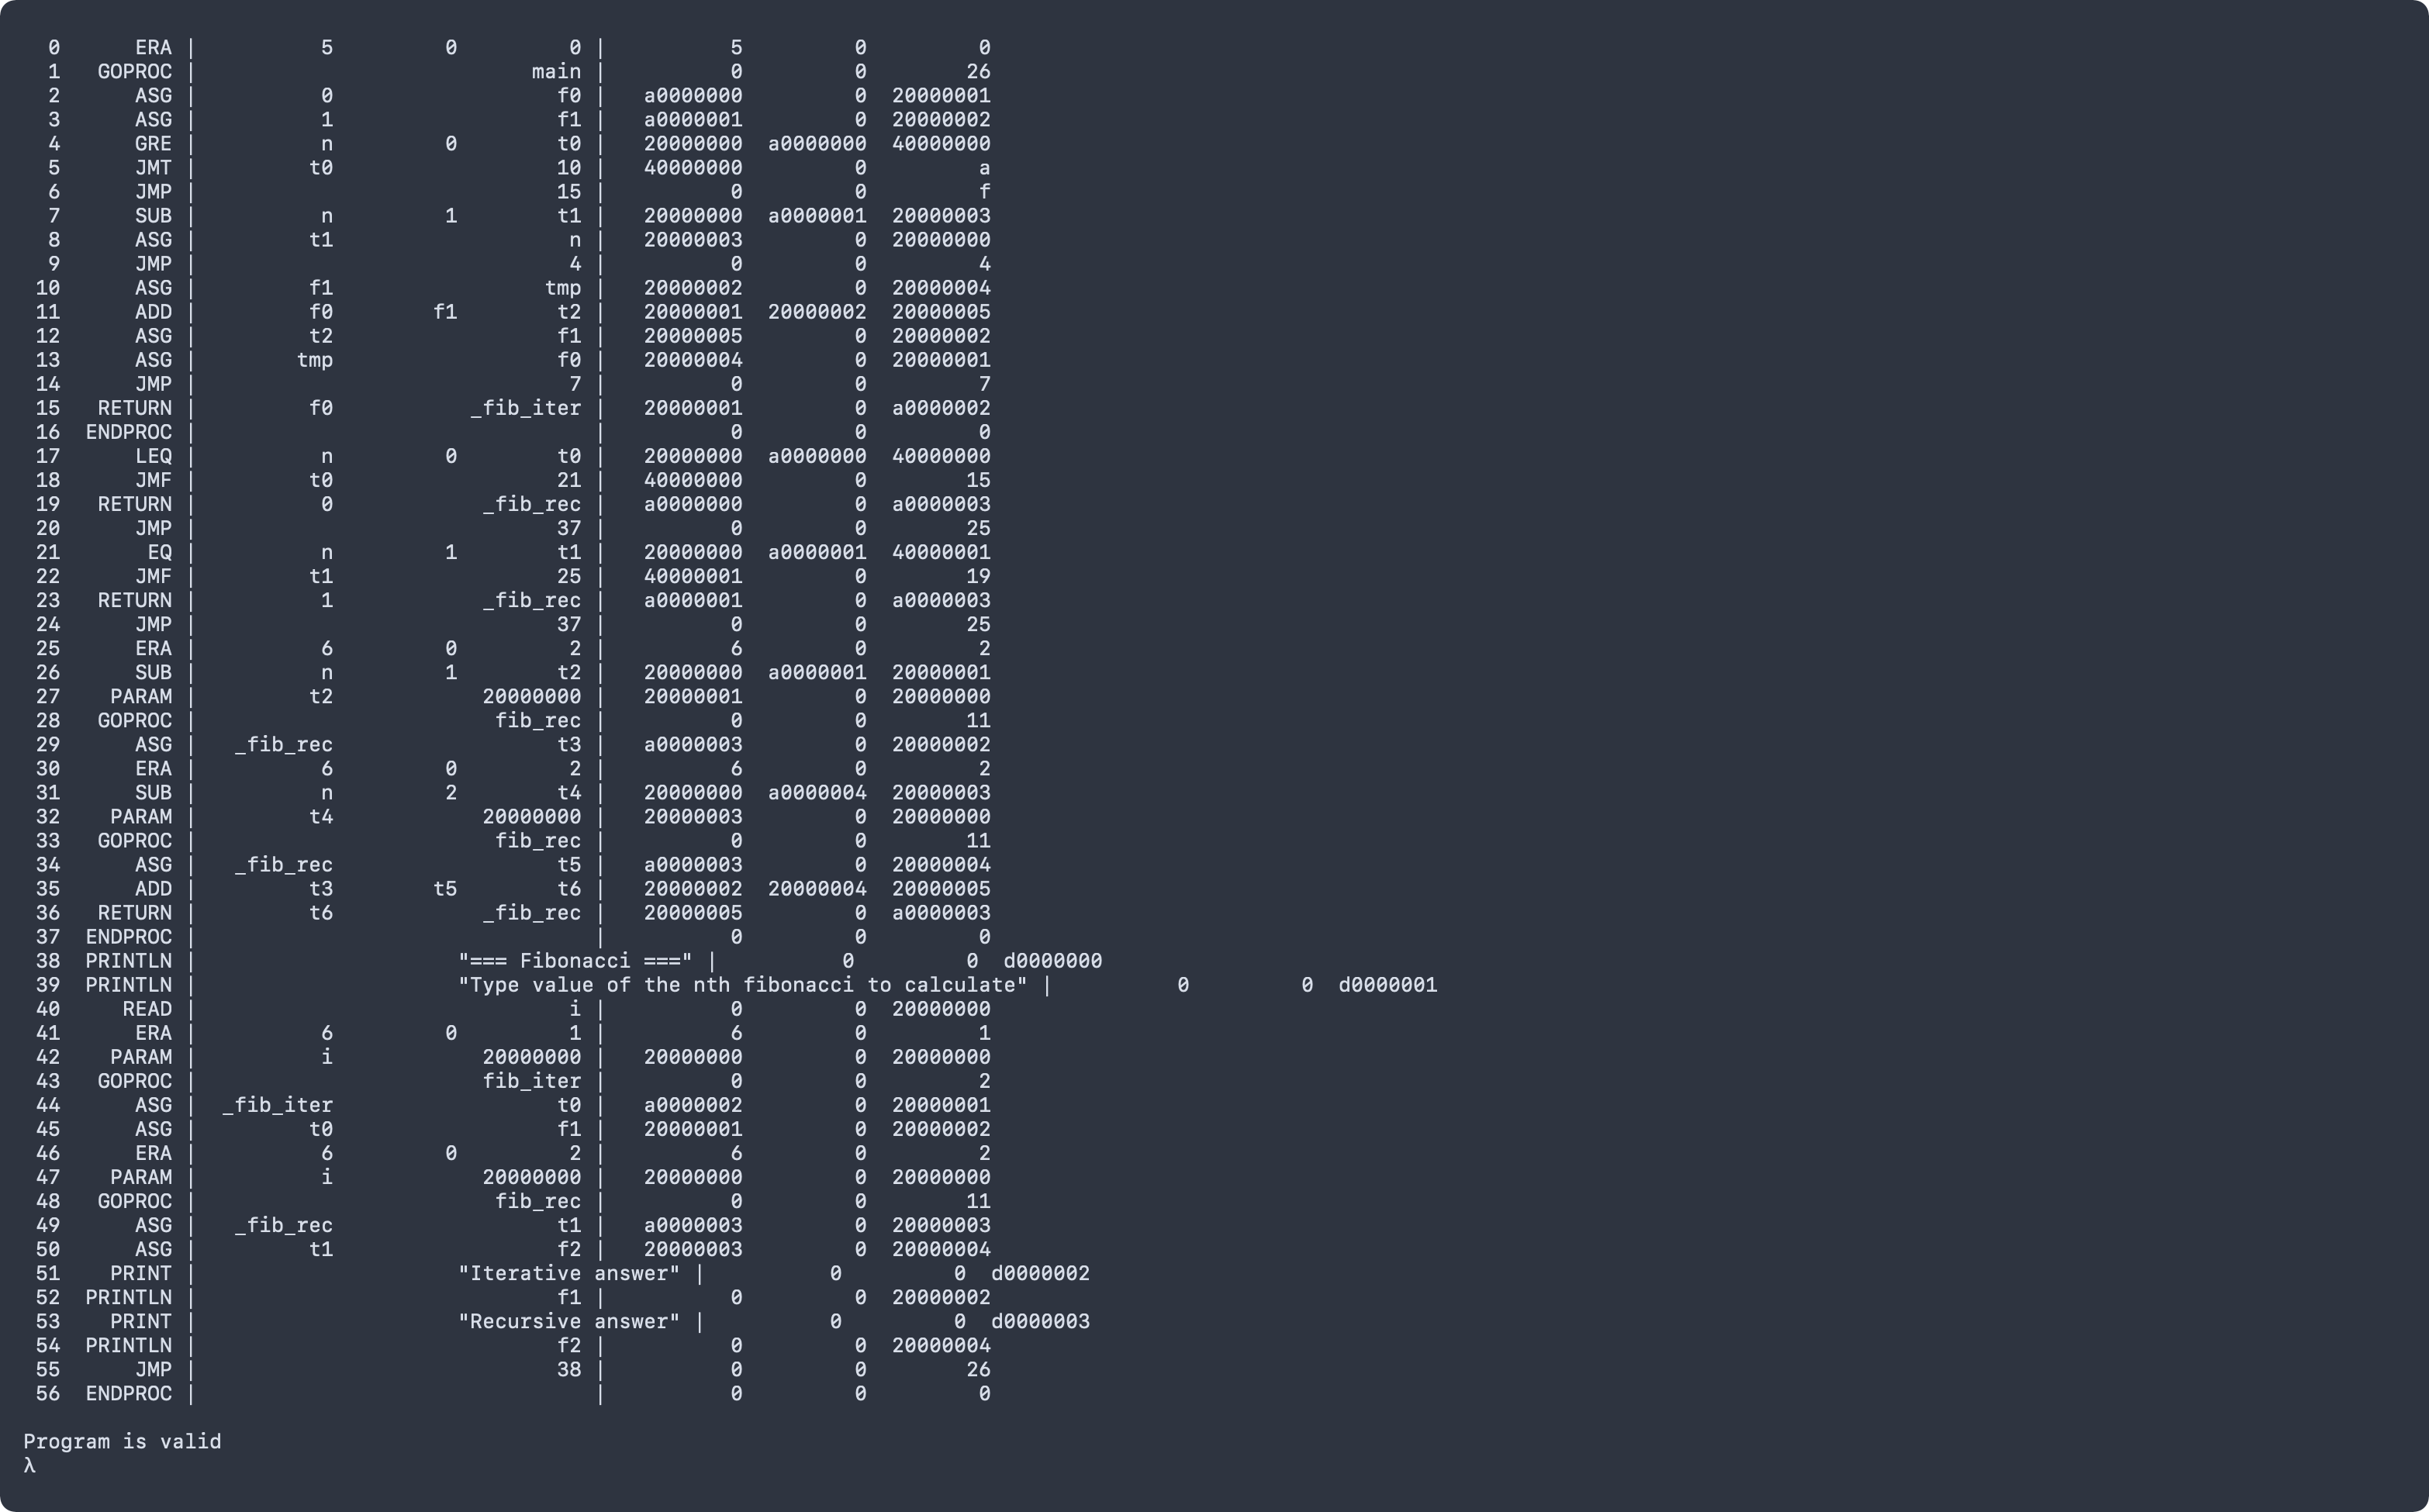
\includegraphics[width=\textwidth]{evidences/fib_ir}
\end{figure}

\begin{figure}[H]
    \centering
    \caption{Program output}
    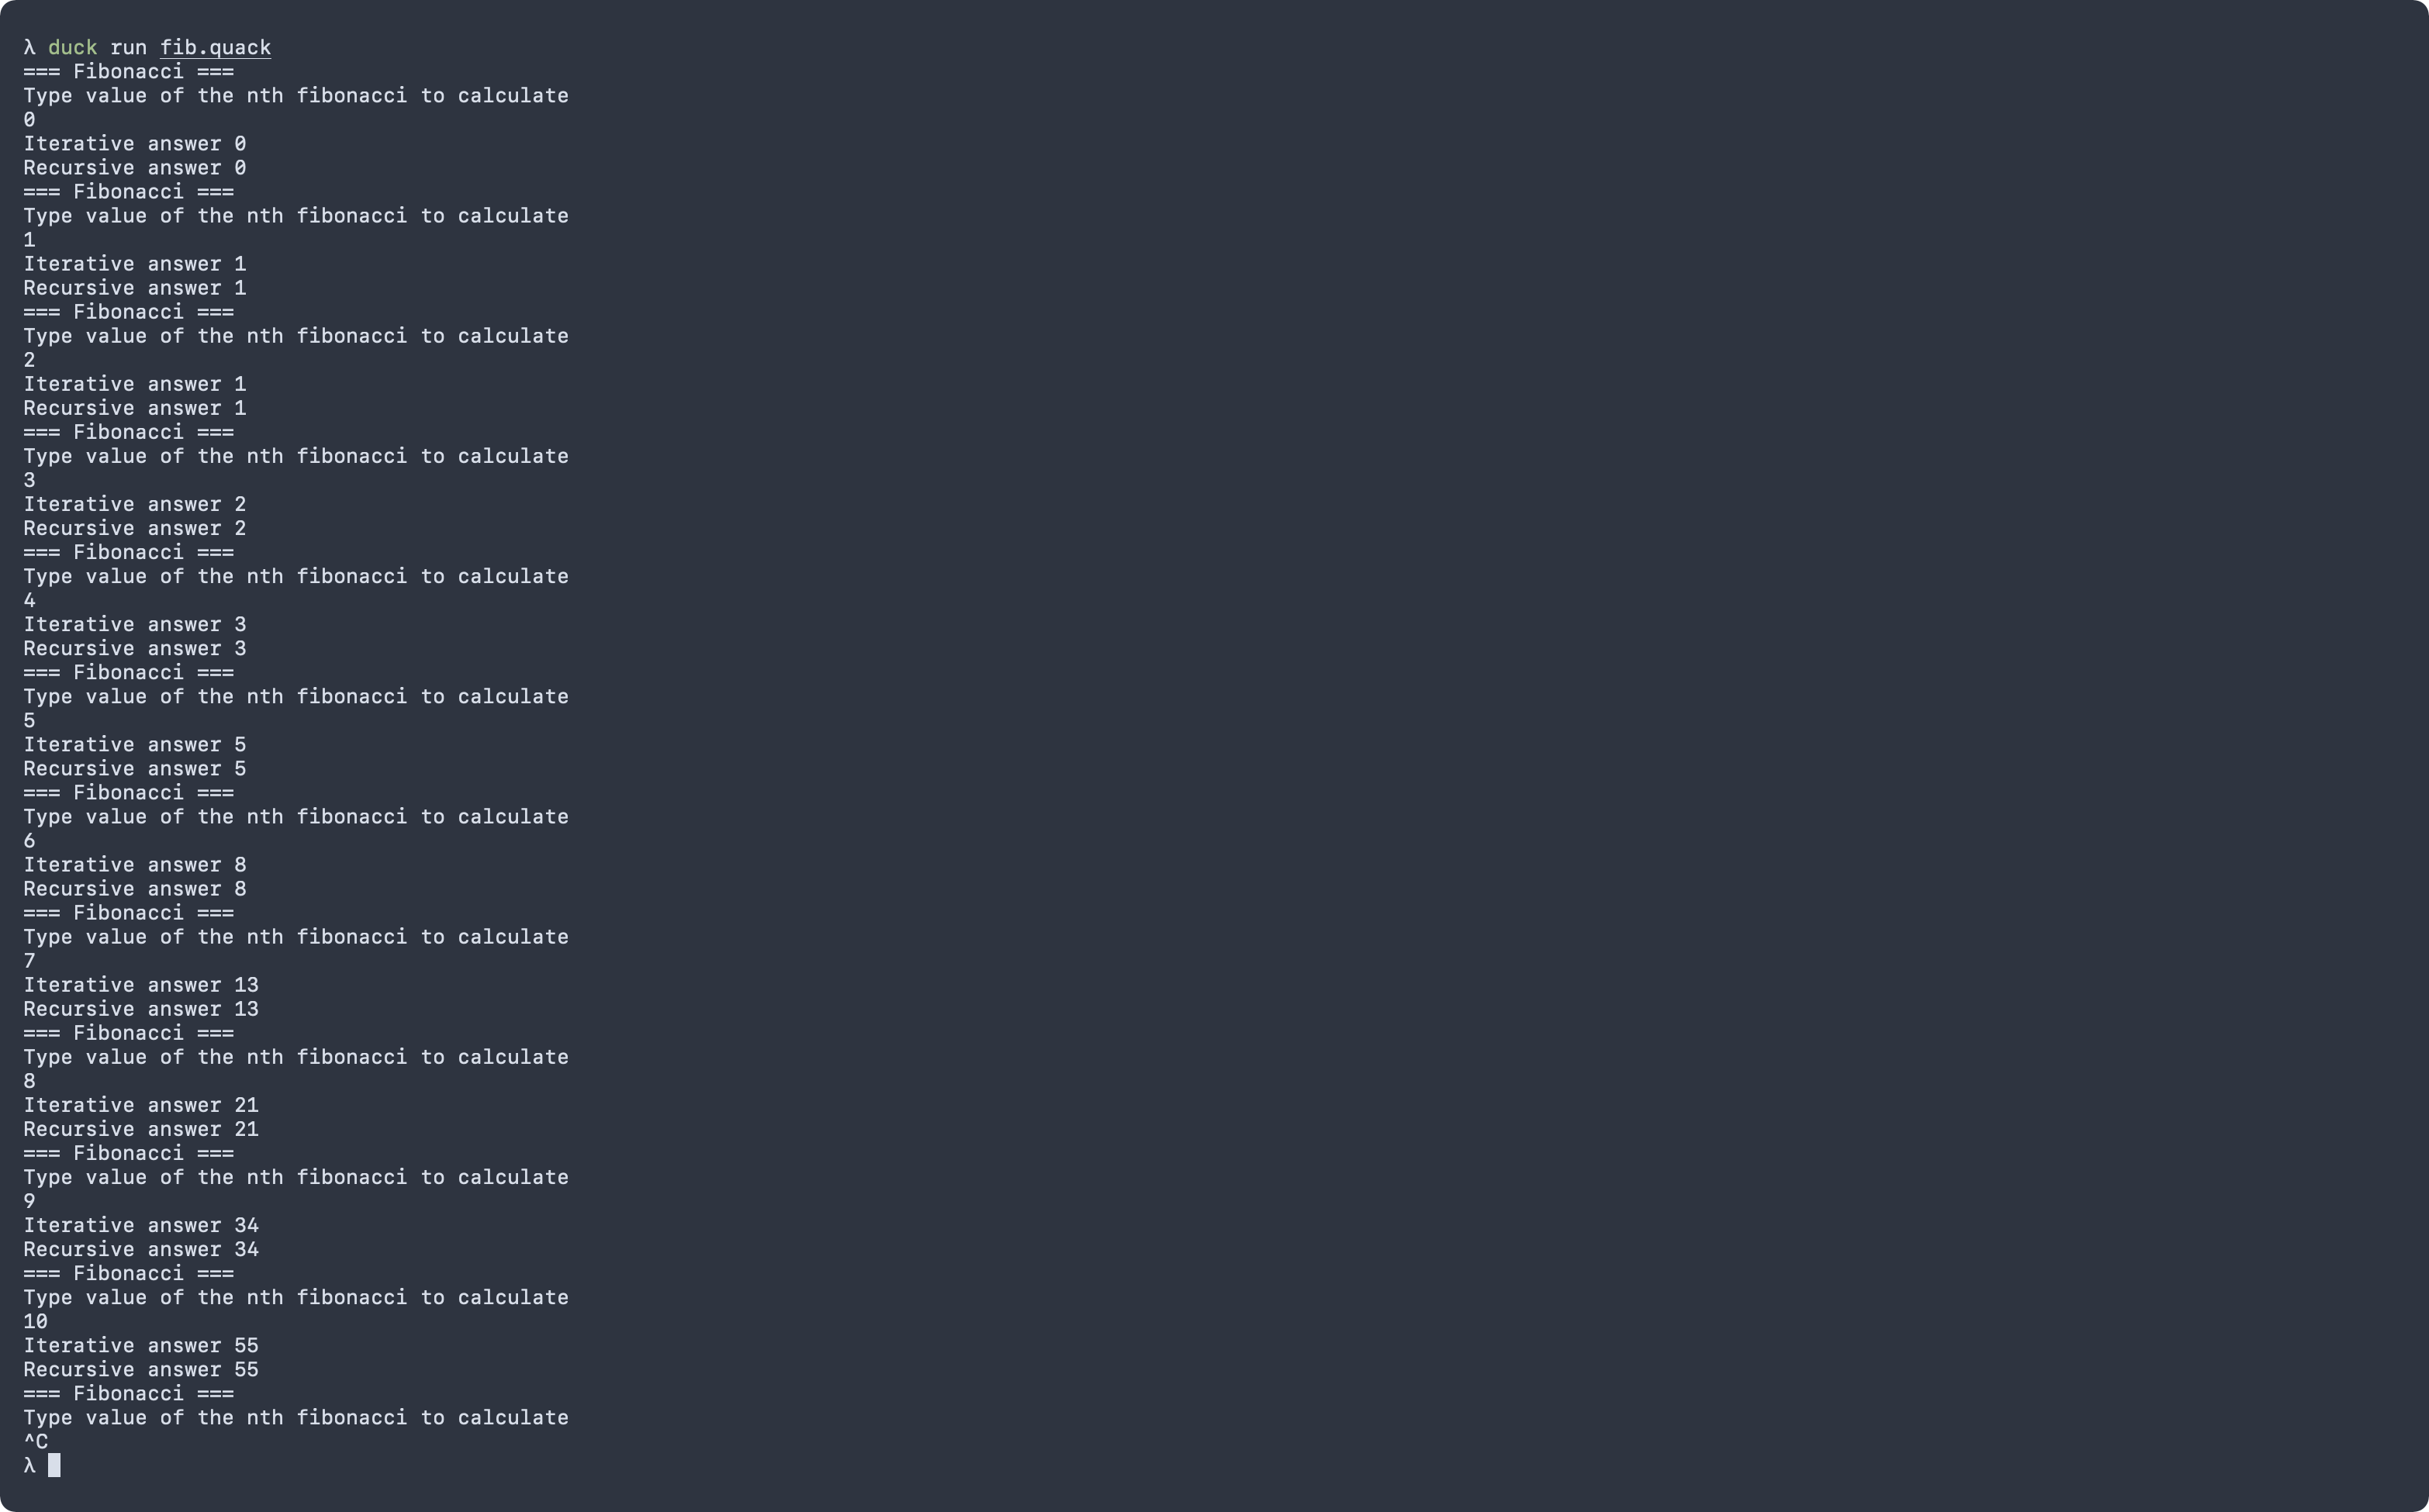
\includegraphics[width=\textwidth]{evidences/fib_output}
\end{figure}

\newpage

\subsection{Find}

\begin{verbatim}
#| Main procedure |#
proc main()
    var array [5]int;
    var x, i, size int;
    var exists bool;
{
    size <- 5;

    print("=== Array ===");

    loop i <- 0; i < size; i <- i + 1 {
        array[i] <- read("Type value at position", i);
    }

    print("=== Value to find ===");

    x <- read("Type value to find");

    loop i <- 0; i < size; i <- i + 1 {
        if x = array[i] {
            exists <- true;
            break;
        }
    }

    print("=== Result ===");

    if exists {
        print("Value", x, "was found in array at position", i);
    } else {
        print("Value", x, "was not found in array");
    }
}
\end{verbatim}

\begin{figure}[H]
    \centering
    \caption{Generated IR code}
    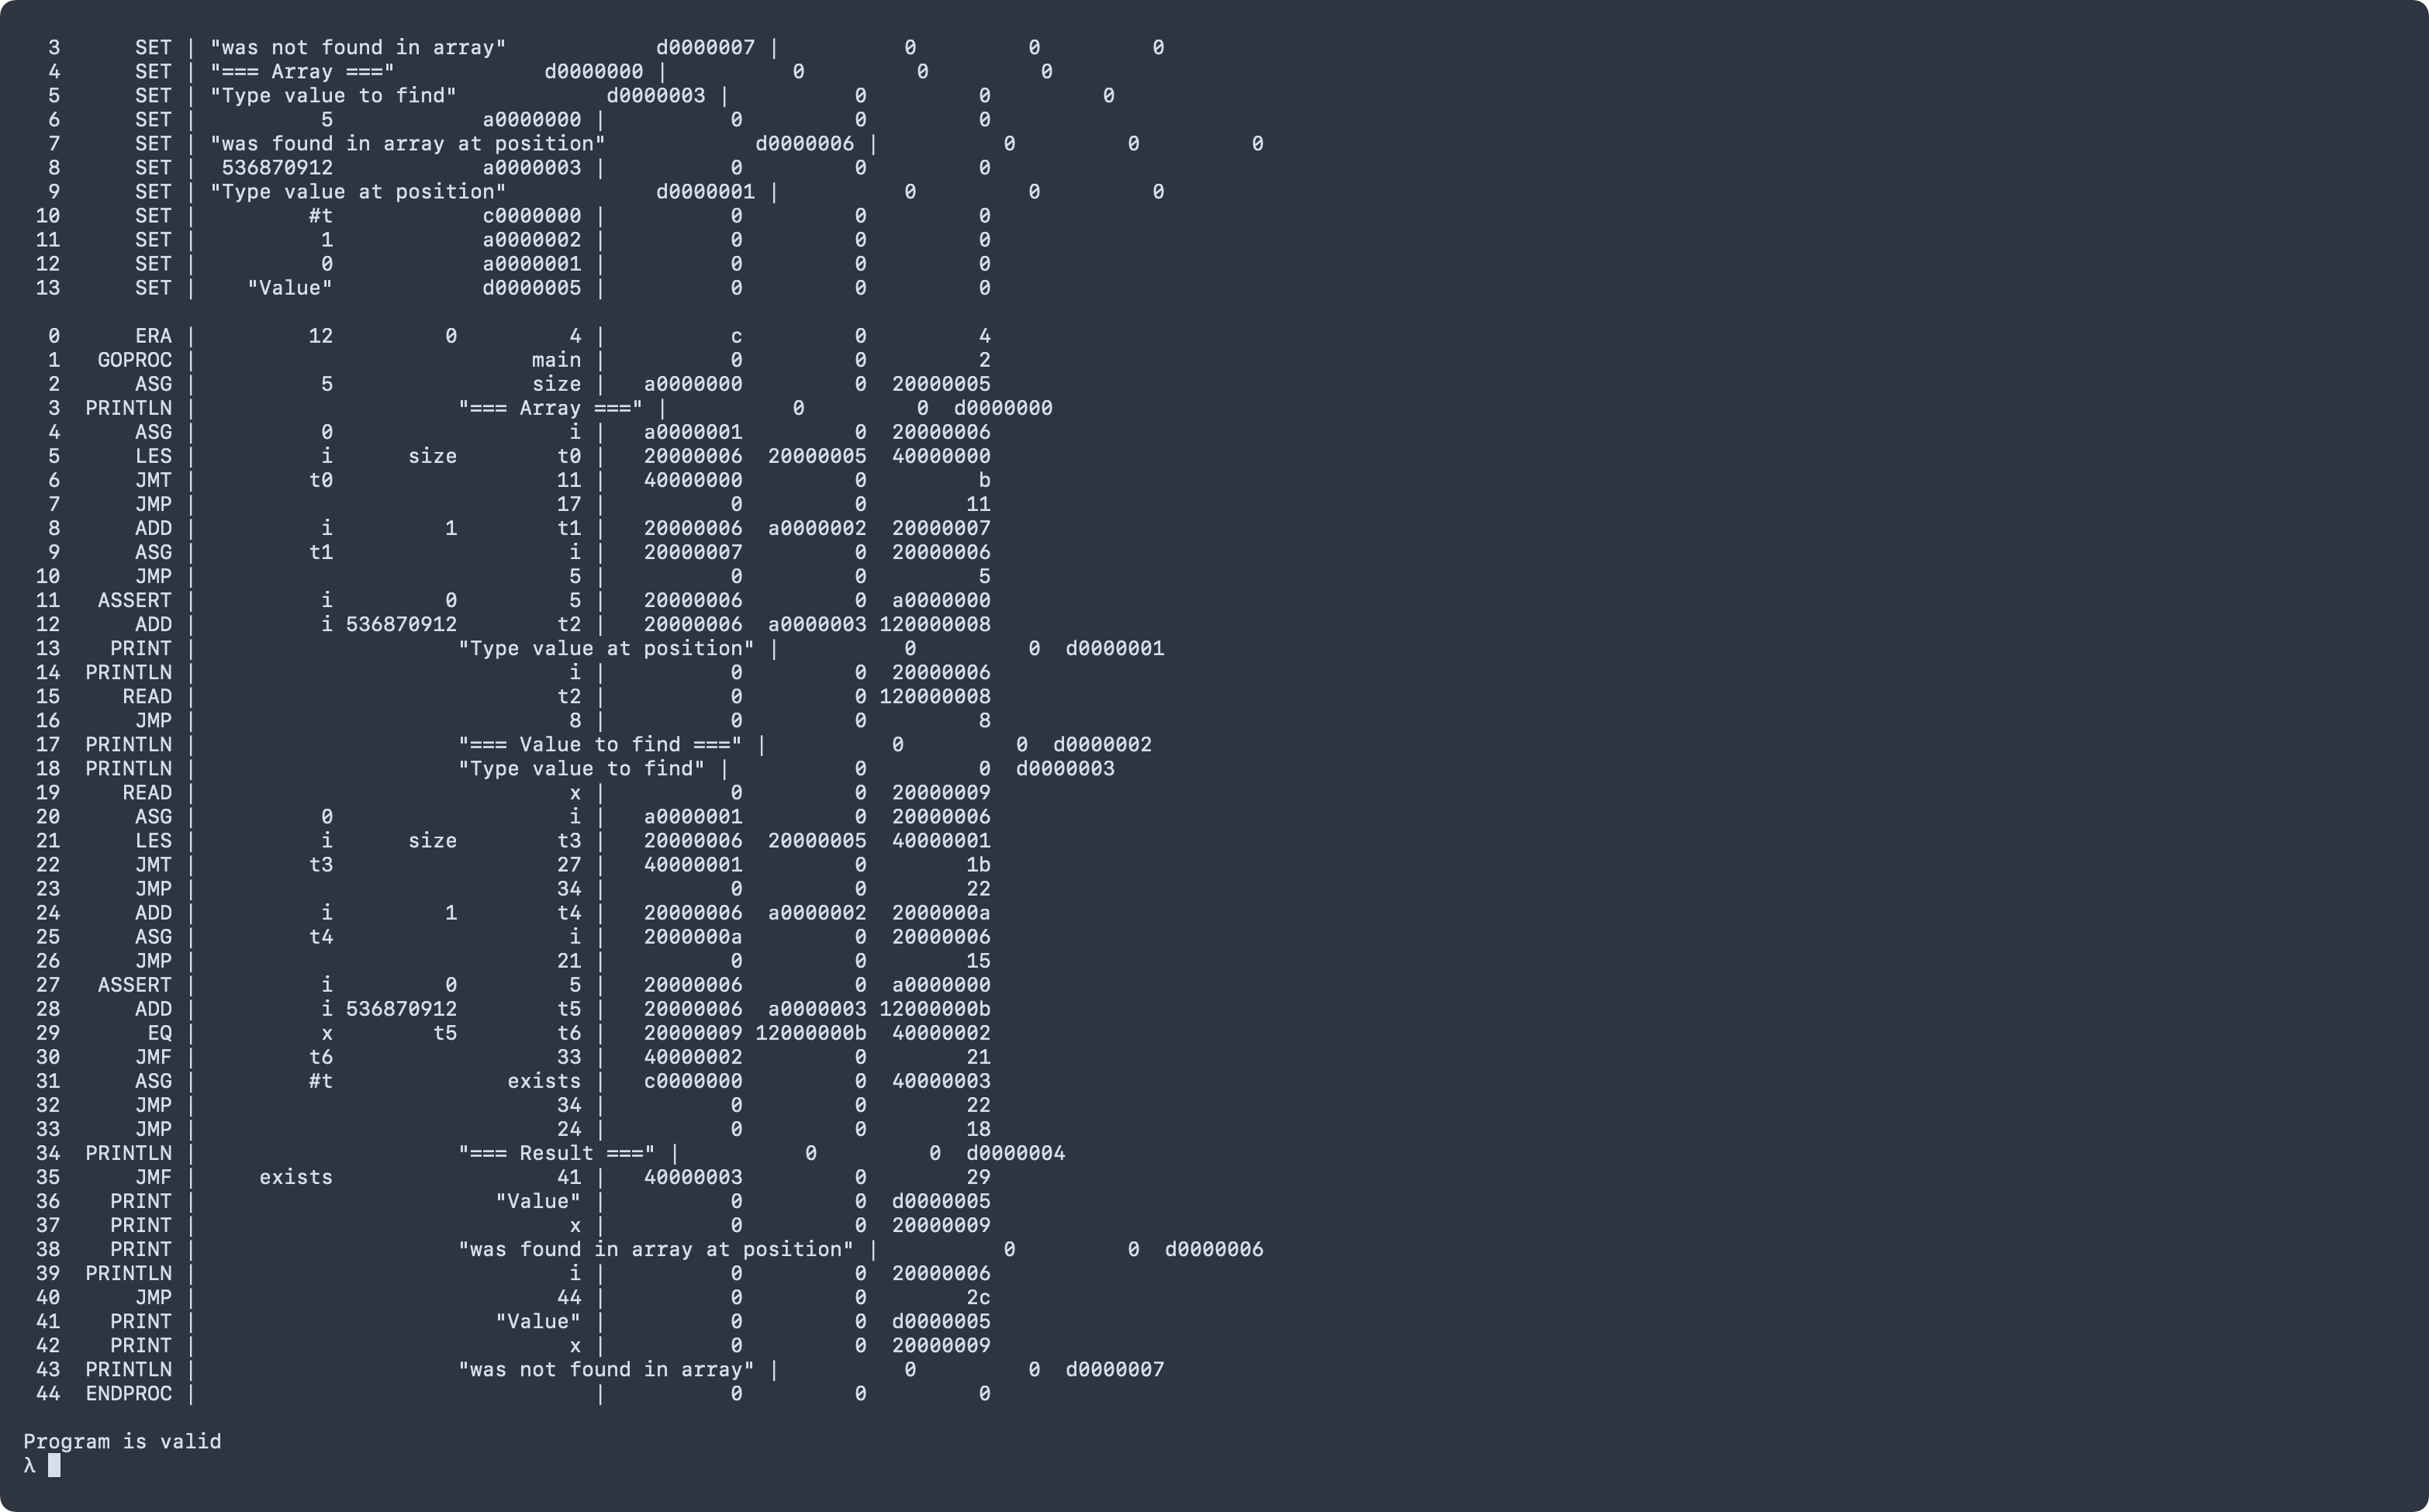
\includegraphics[width=\textwidth]{evidences/find_ir}
\end{figure}

\begin{figure}[H]
    \centering
    \caption{Program output}
    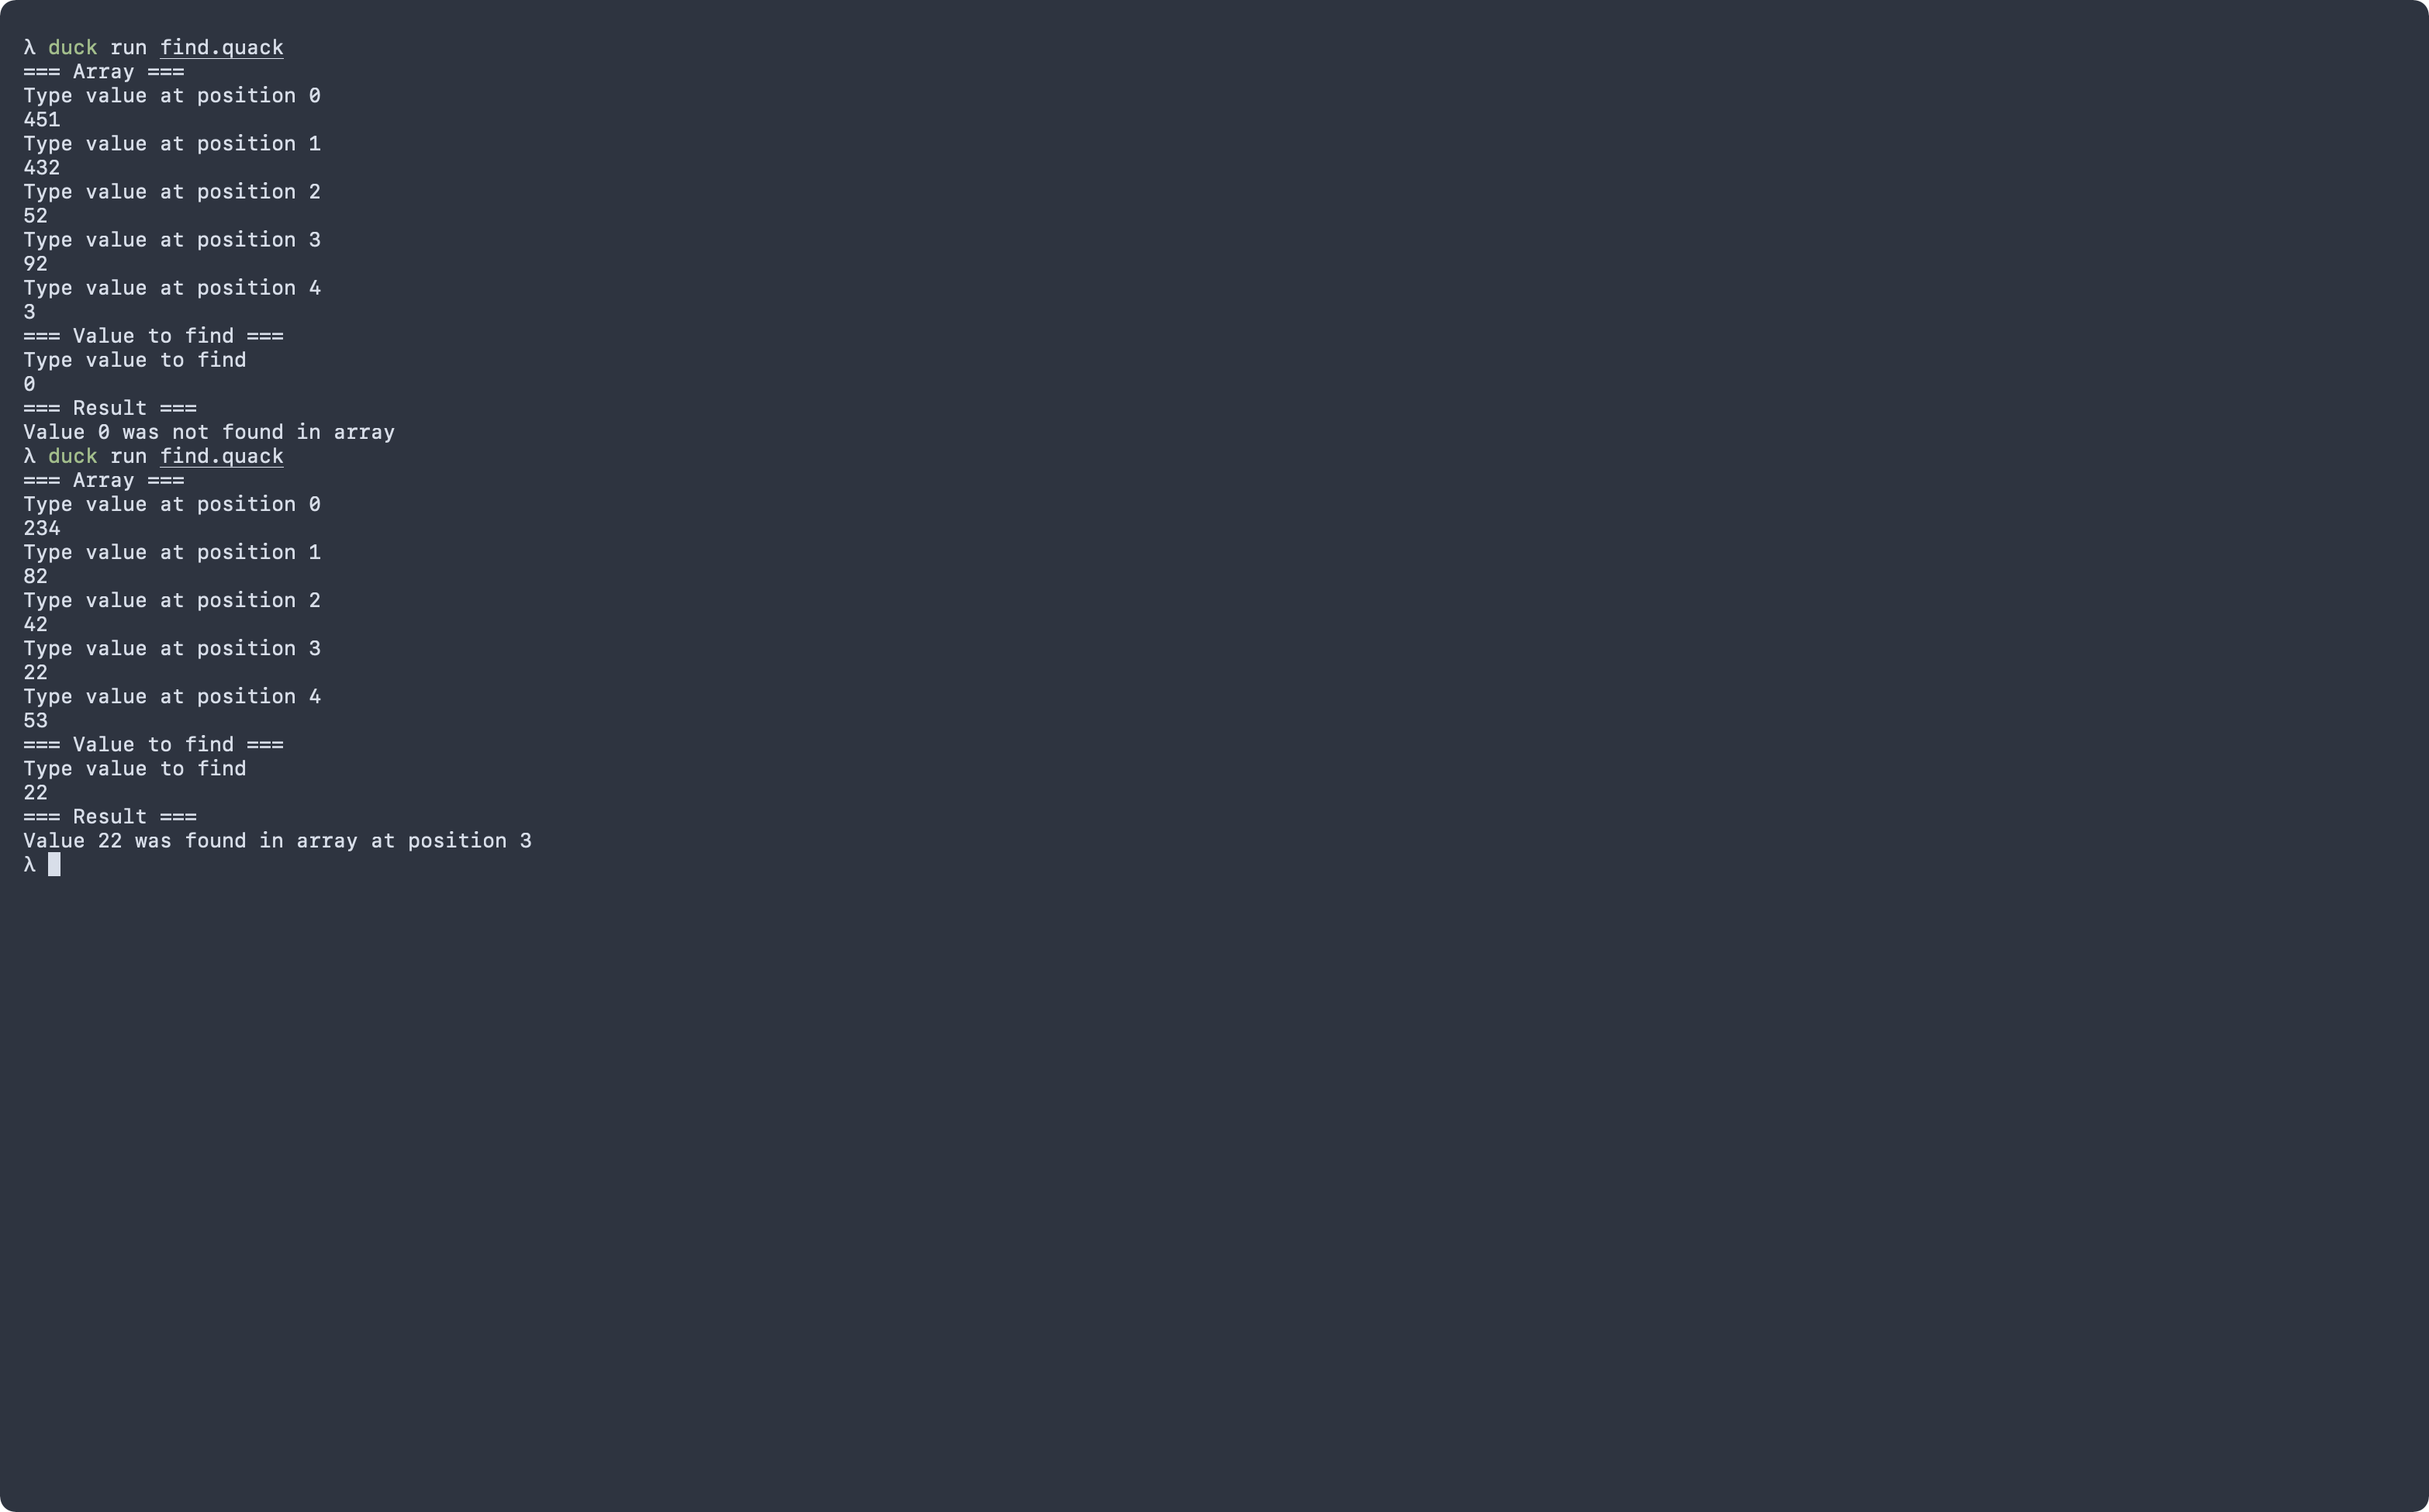
\includegraphics[width=\textwidth]{evidences/find_output}
\end{figure}

\newpage

\subsection{Sort}

\begin{verbatim}
#| Main procedure |#
proc main()
    var array [5]int;
    var i, j, tmp, size int;
    var is_sorted bool;
{
    size <- 5;

    print("=== Fill array ===");

    loop i <- 0; i < size; i <- i + 1 {
        array[i] <- read("Type value at position", i);
    }

#| Bubble sort |#
    loop i <- 0; i < size - 1; i <- i + 1 {
        is_sorted <- true;

        loop j <- i + 1; j < size; j <- j + 1 {
            if array[i] > array[j] {
                tmp <- array[i];
                array[i] <- array[j];
                array[j] <- tmp;
                is_sorted <- false;
            }
        }

        if is_sorted {
            break;
        }
    }
    
    print("=== Sorted array ===");
    print(array);
}
\end{verbatim}

\begin{figure}[H]
    \centering
    \caption{Generated IR code}
    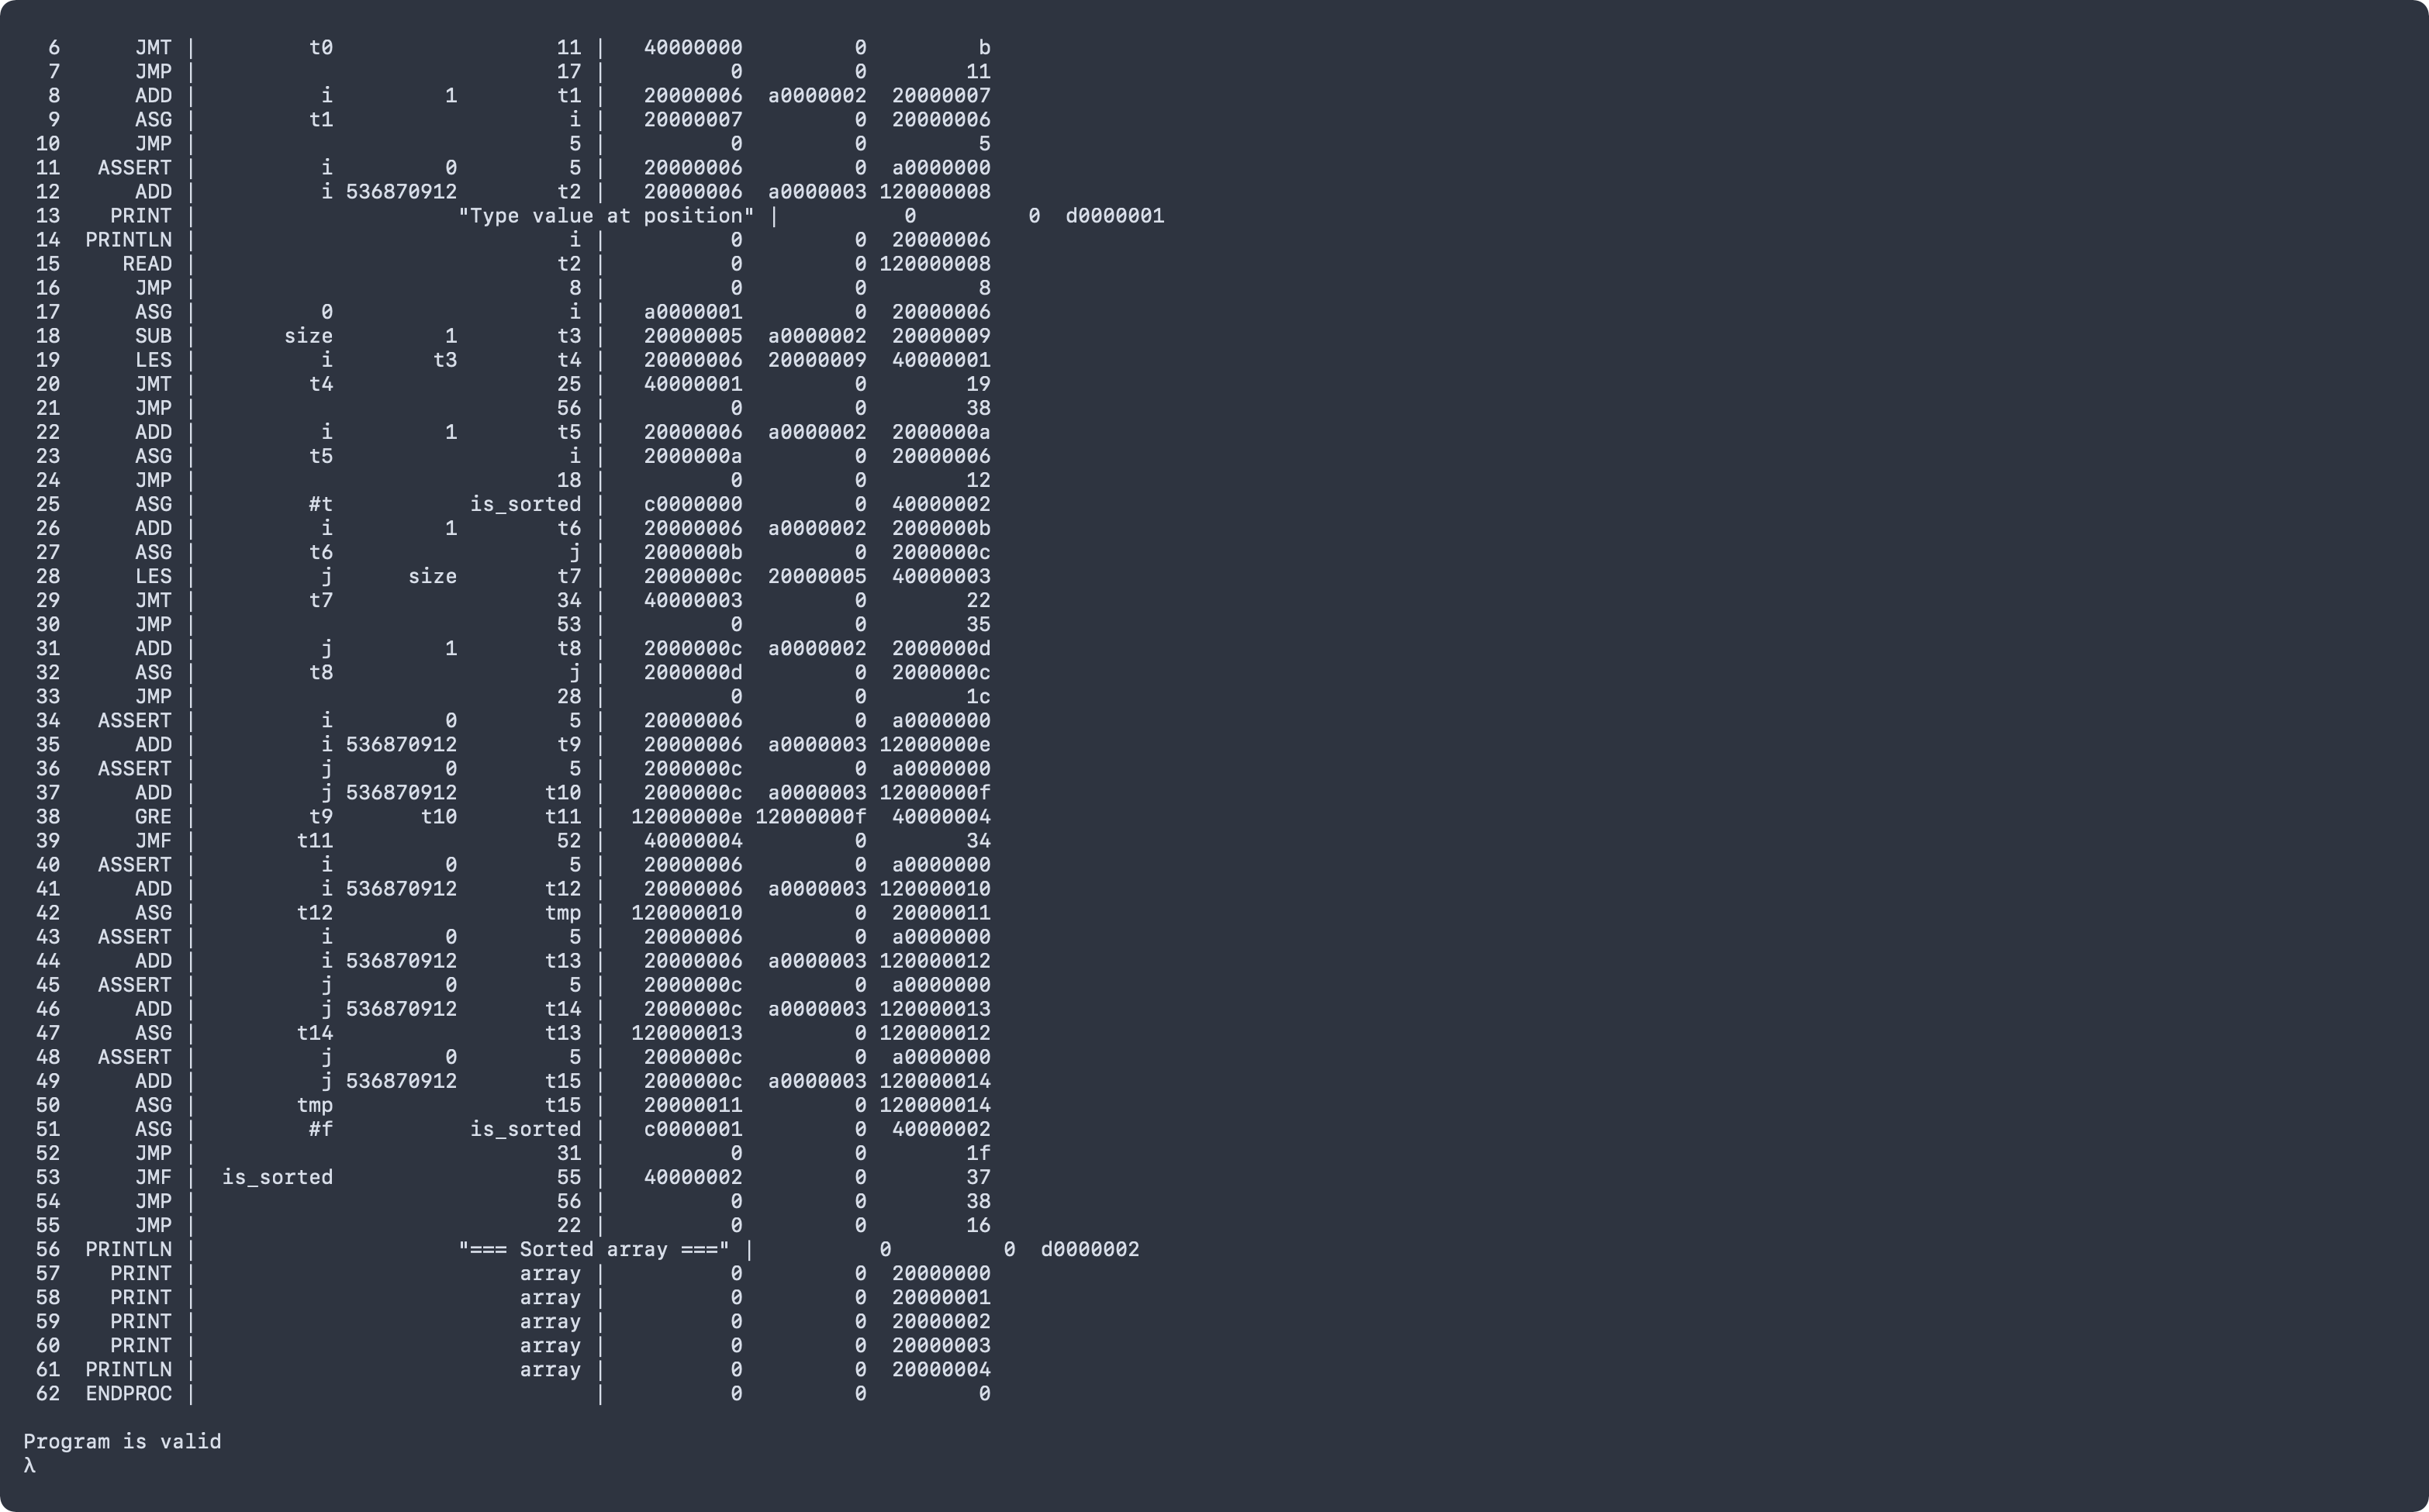
\includegraphics[width=\textwidth]{evidences/sort_ir}
\end{figure}

\begin{figure}[H]
    \centering
    \caption{Program output}
    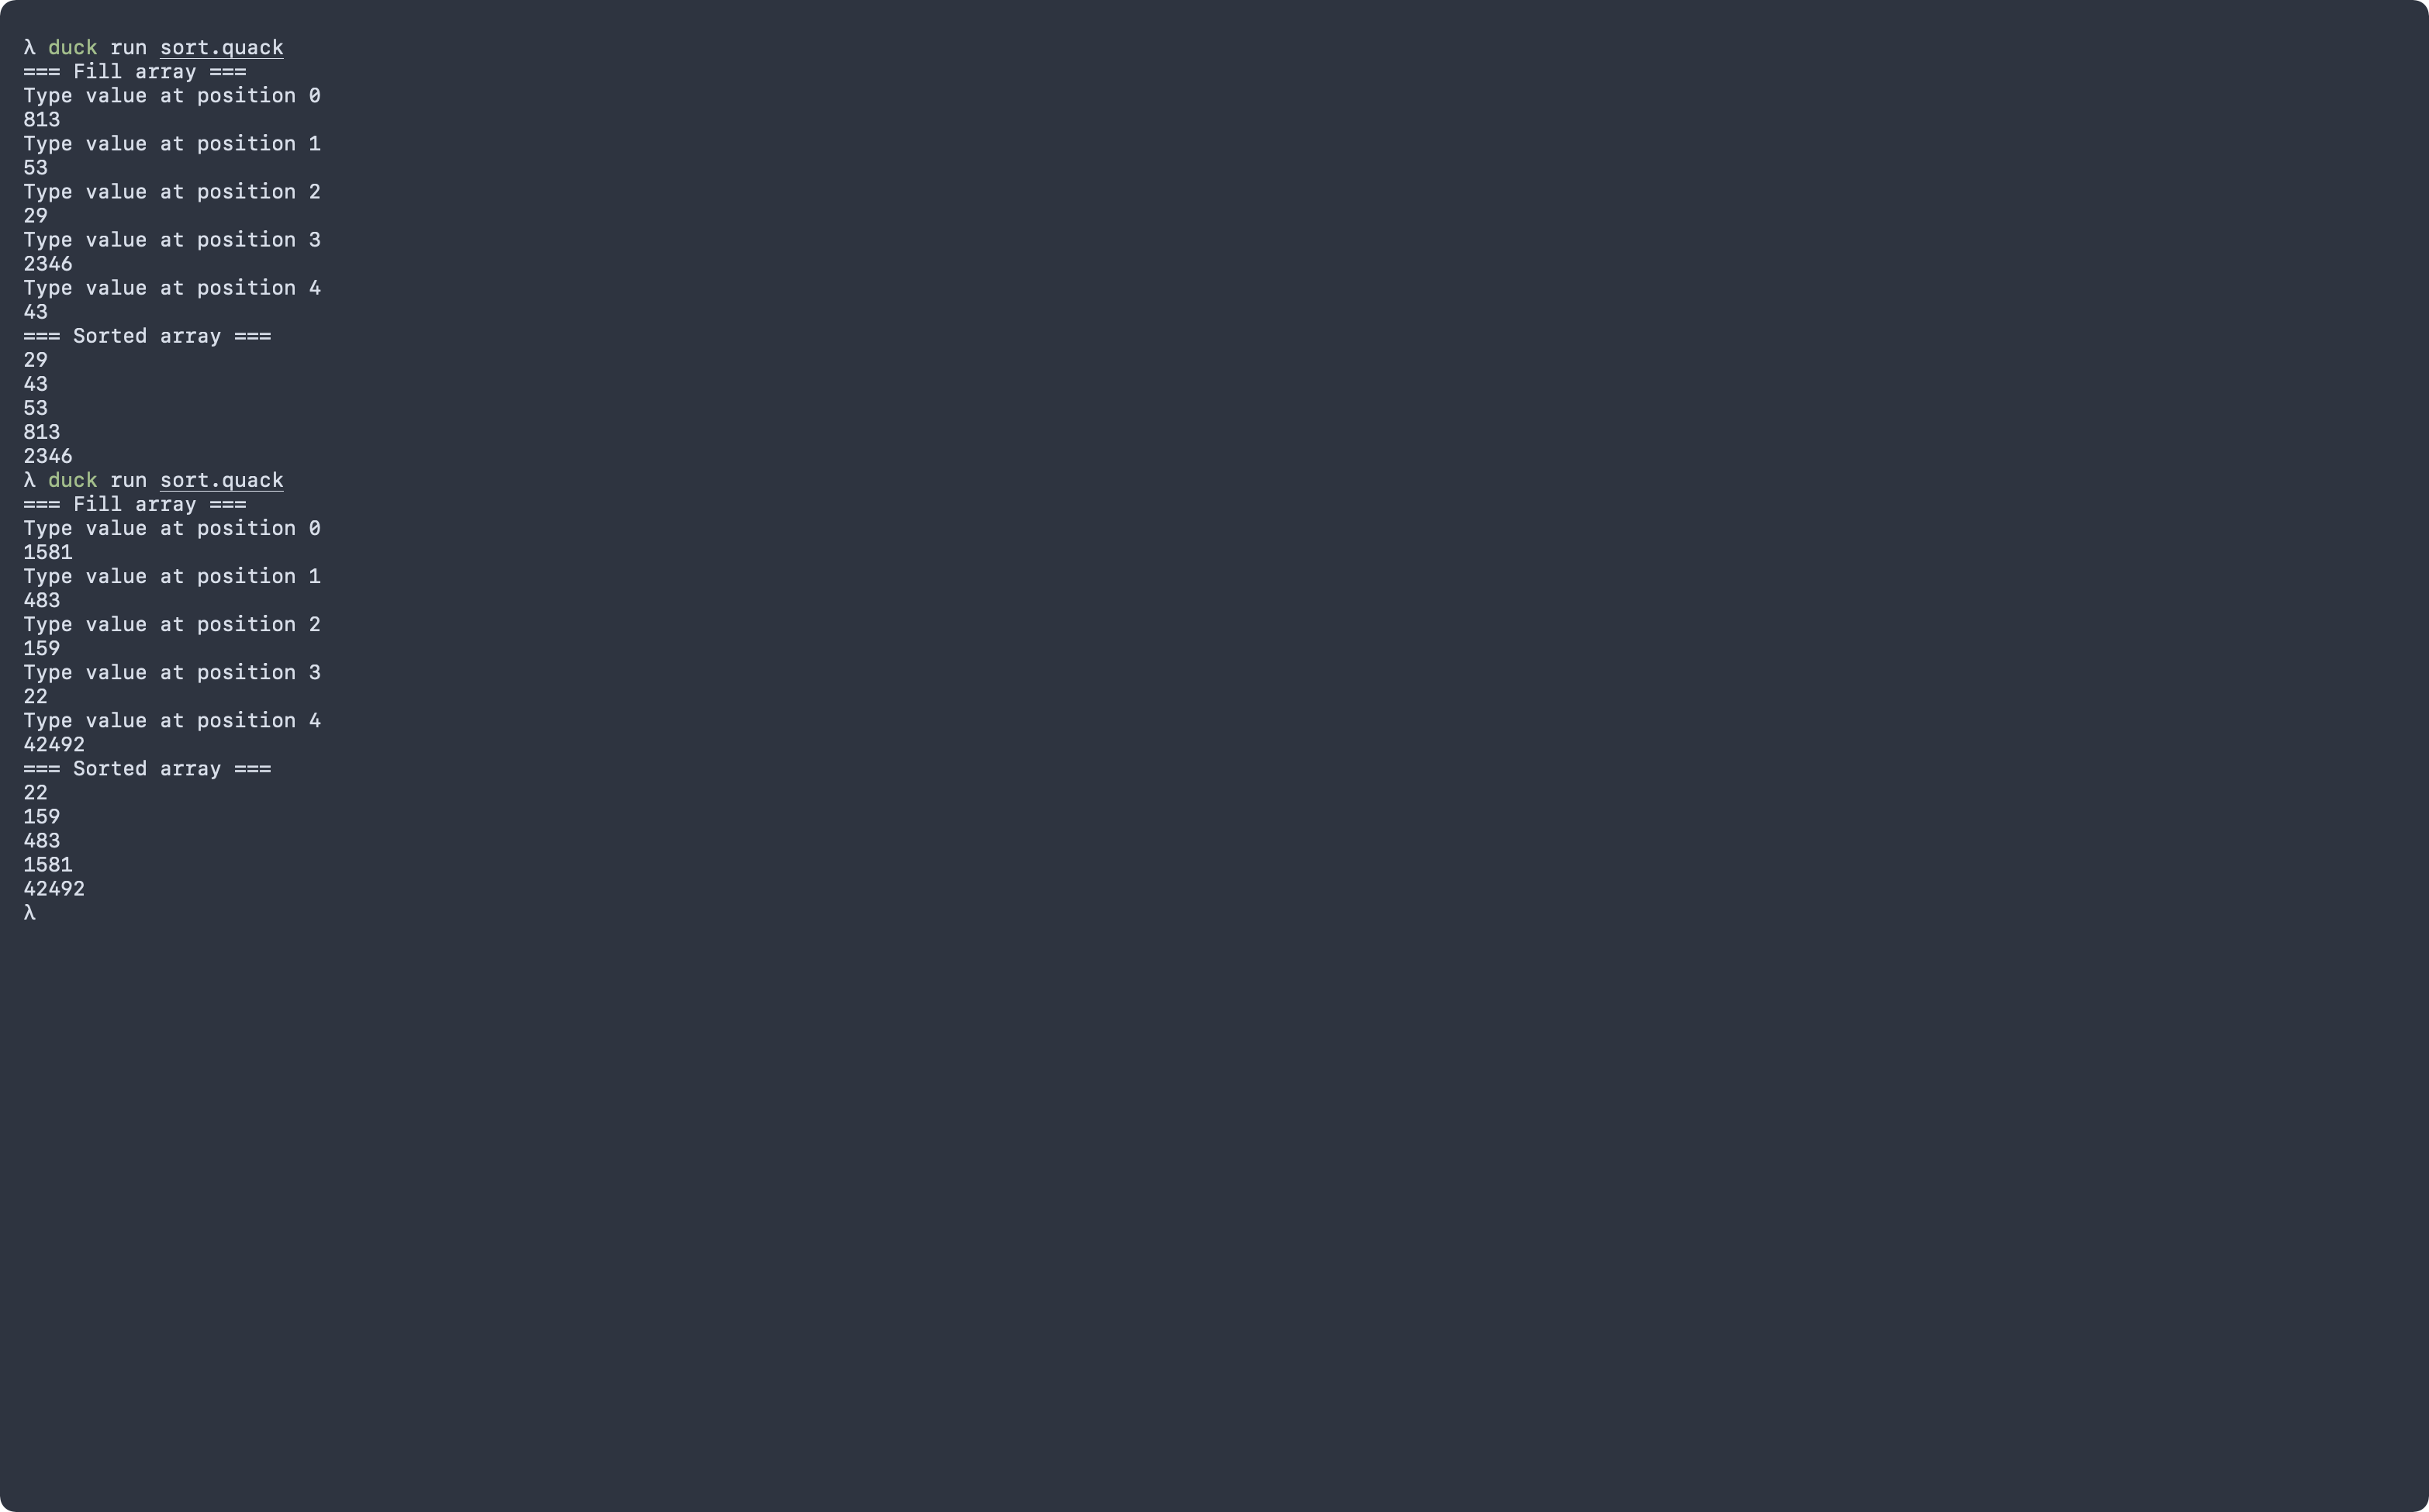
\includegraphics[width=\textwidth]{evidences/sort_output}
\end{figure}

\newpage

\subsection{Matrix multiplication}

\begin{verbatim}
#| Main procedure |#

proc main()
    var a [2][2]int;
    var b [2][2]int;
    var c [2][2]int;
    var i, j, k, I, J, K int;
{
    I <- 2;
    J <- 2;
    K <- 2;

    print("=== Fill matrices ===");

    loop i <- 0; i < I; i <- i + 1 {
        loop k <- 0; k < K; k <- k + 1 {
            a[i][k] <- read("Type value at a[", i, "][", k, "]");
        }
    }

    loop k <- 0; k < K; k <- k + 1 {
        loop j <- 0; j < J; j <- j + 1 {
            b[k][j] <- read("Type value at b[", k, "][", j, "]");
        }
    }

    loop i <- 0; i < I; i <- i + 1 {
        loop j <- 0; j < J; j <- j + 1 {
            loop k <- 0; k < K; k <- k + 1 {
                c[i][j] <- c[i][j] + a[i][k] * b[k][j];
            }
        }
    }

    print("=== Result ===");
    print(c);
}
\end{verbatim}

\begin{figure}[H]
    \centering
    \caption{Generated IR code}
    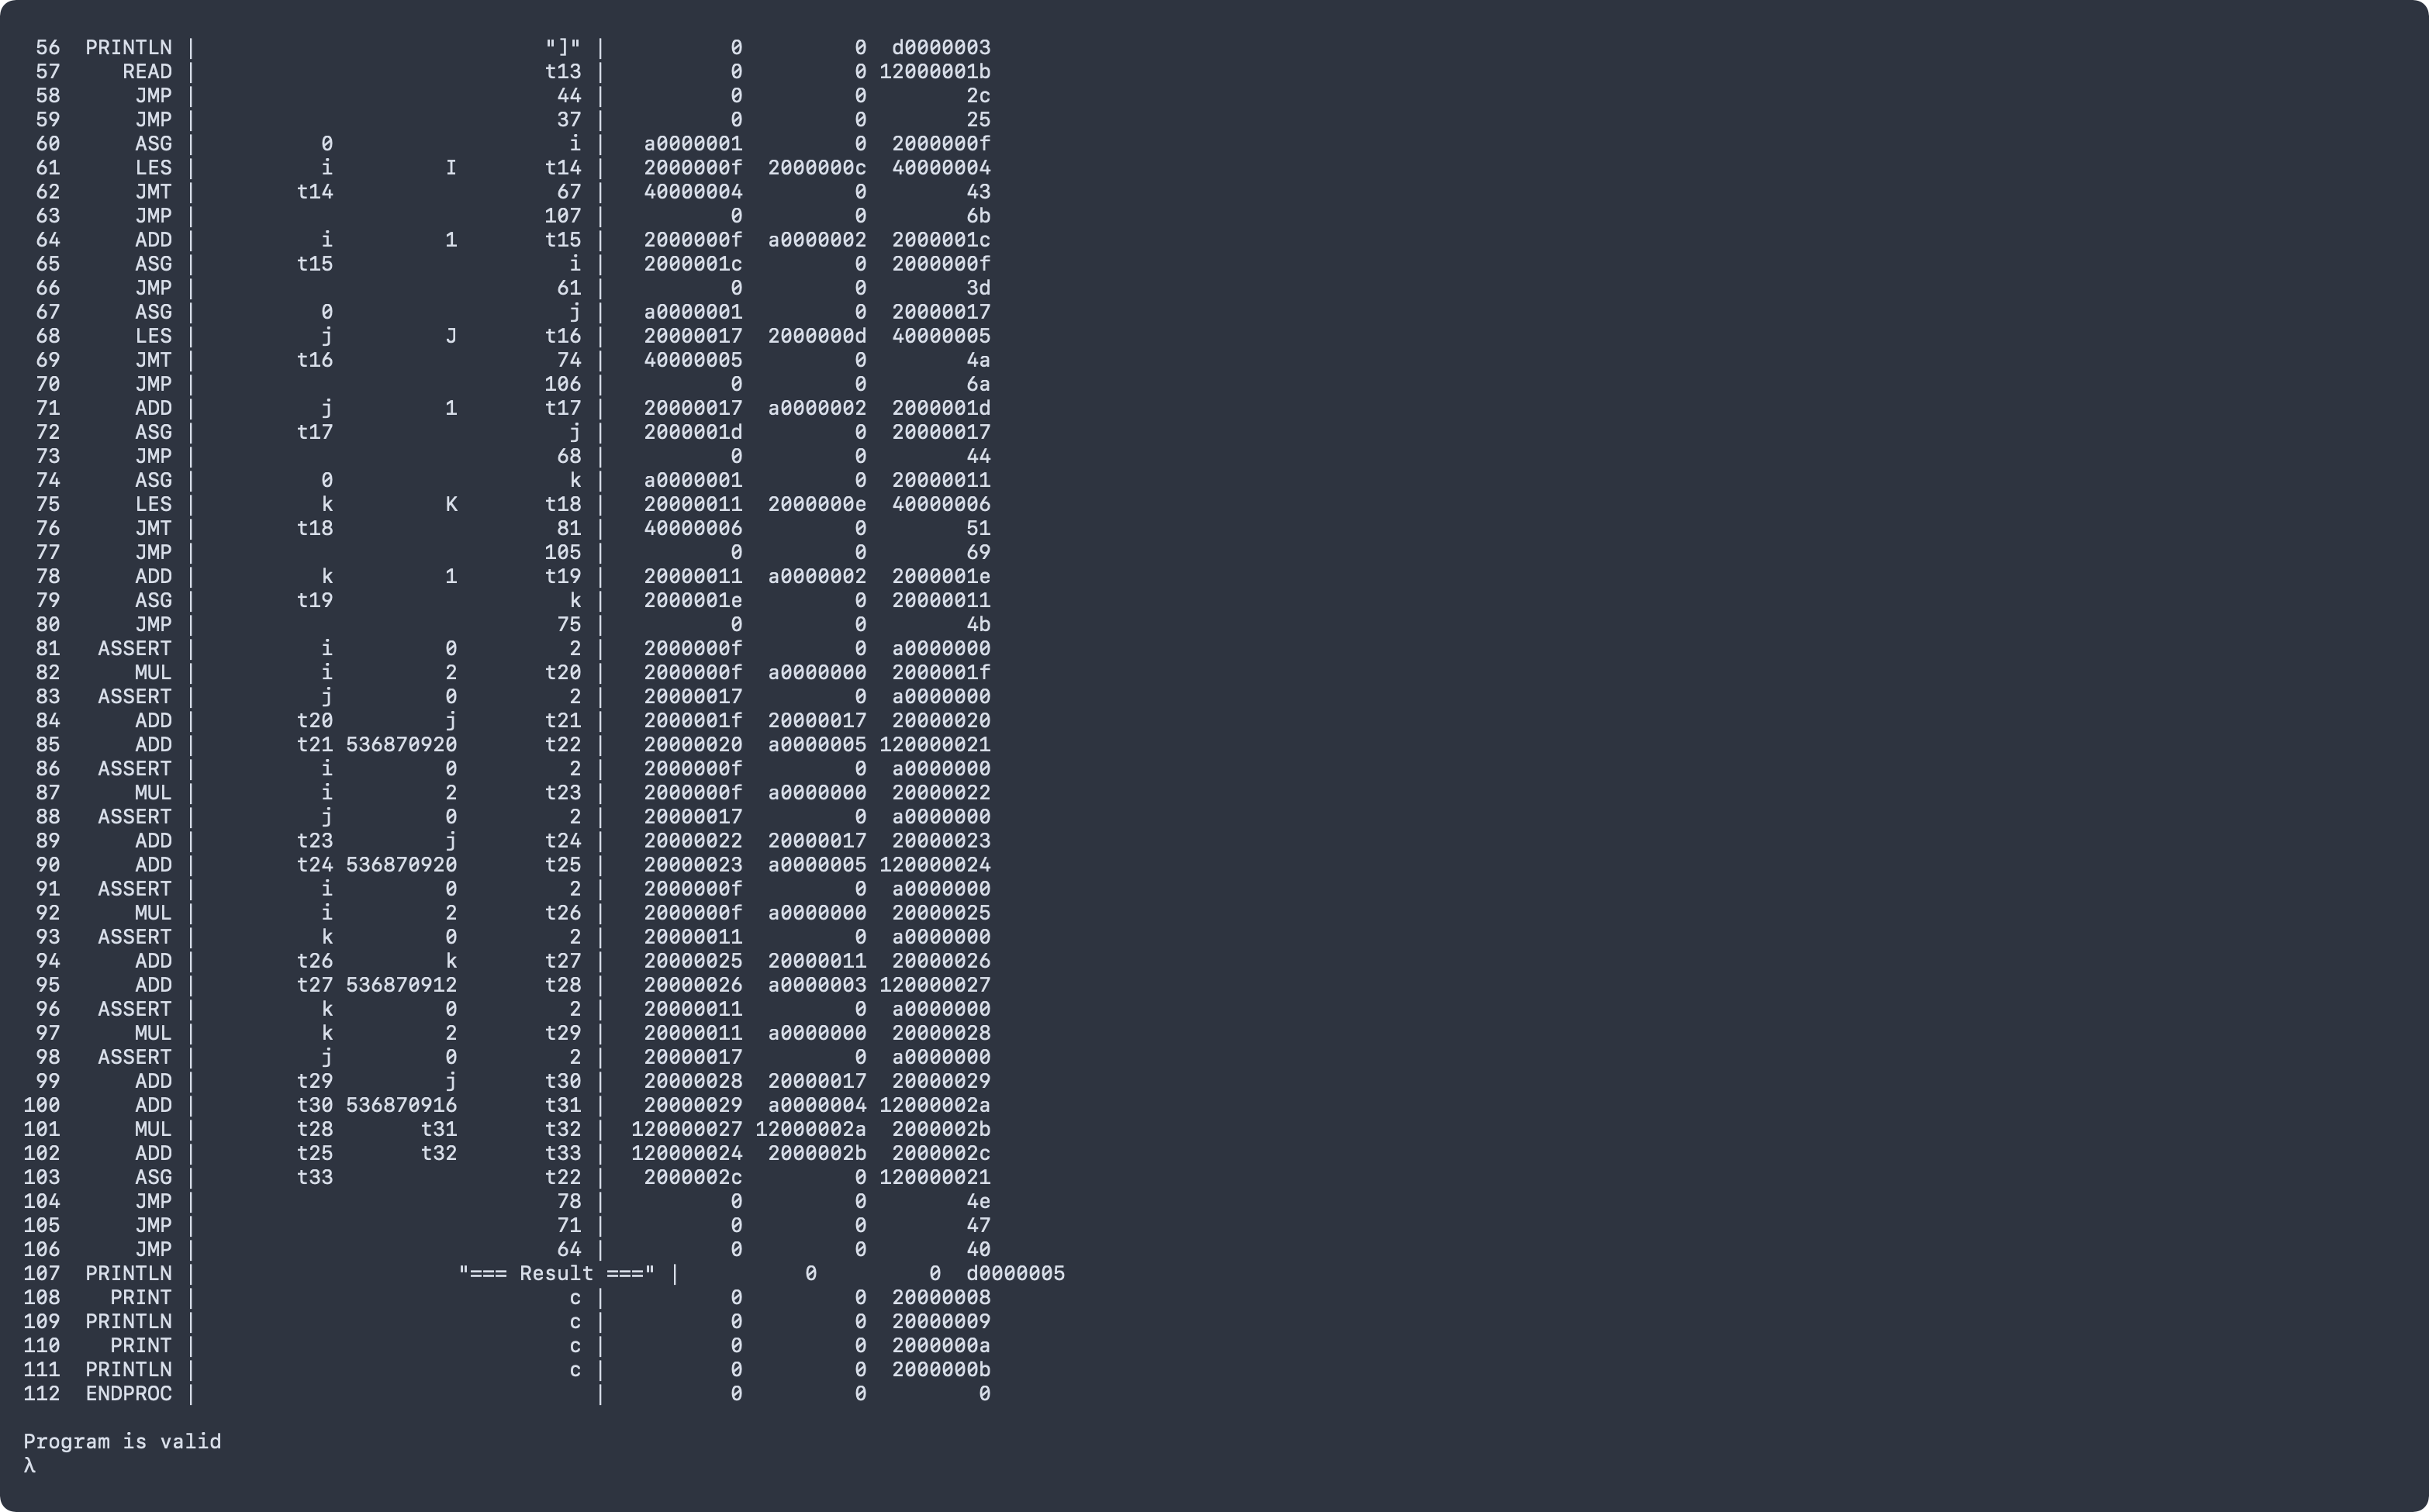
\includegraphics[width=\textwidth]{evidences/mat_mul_ir}
\end{figure}

\begin{figure}[H]
    \centering
    \caption{Program output}
    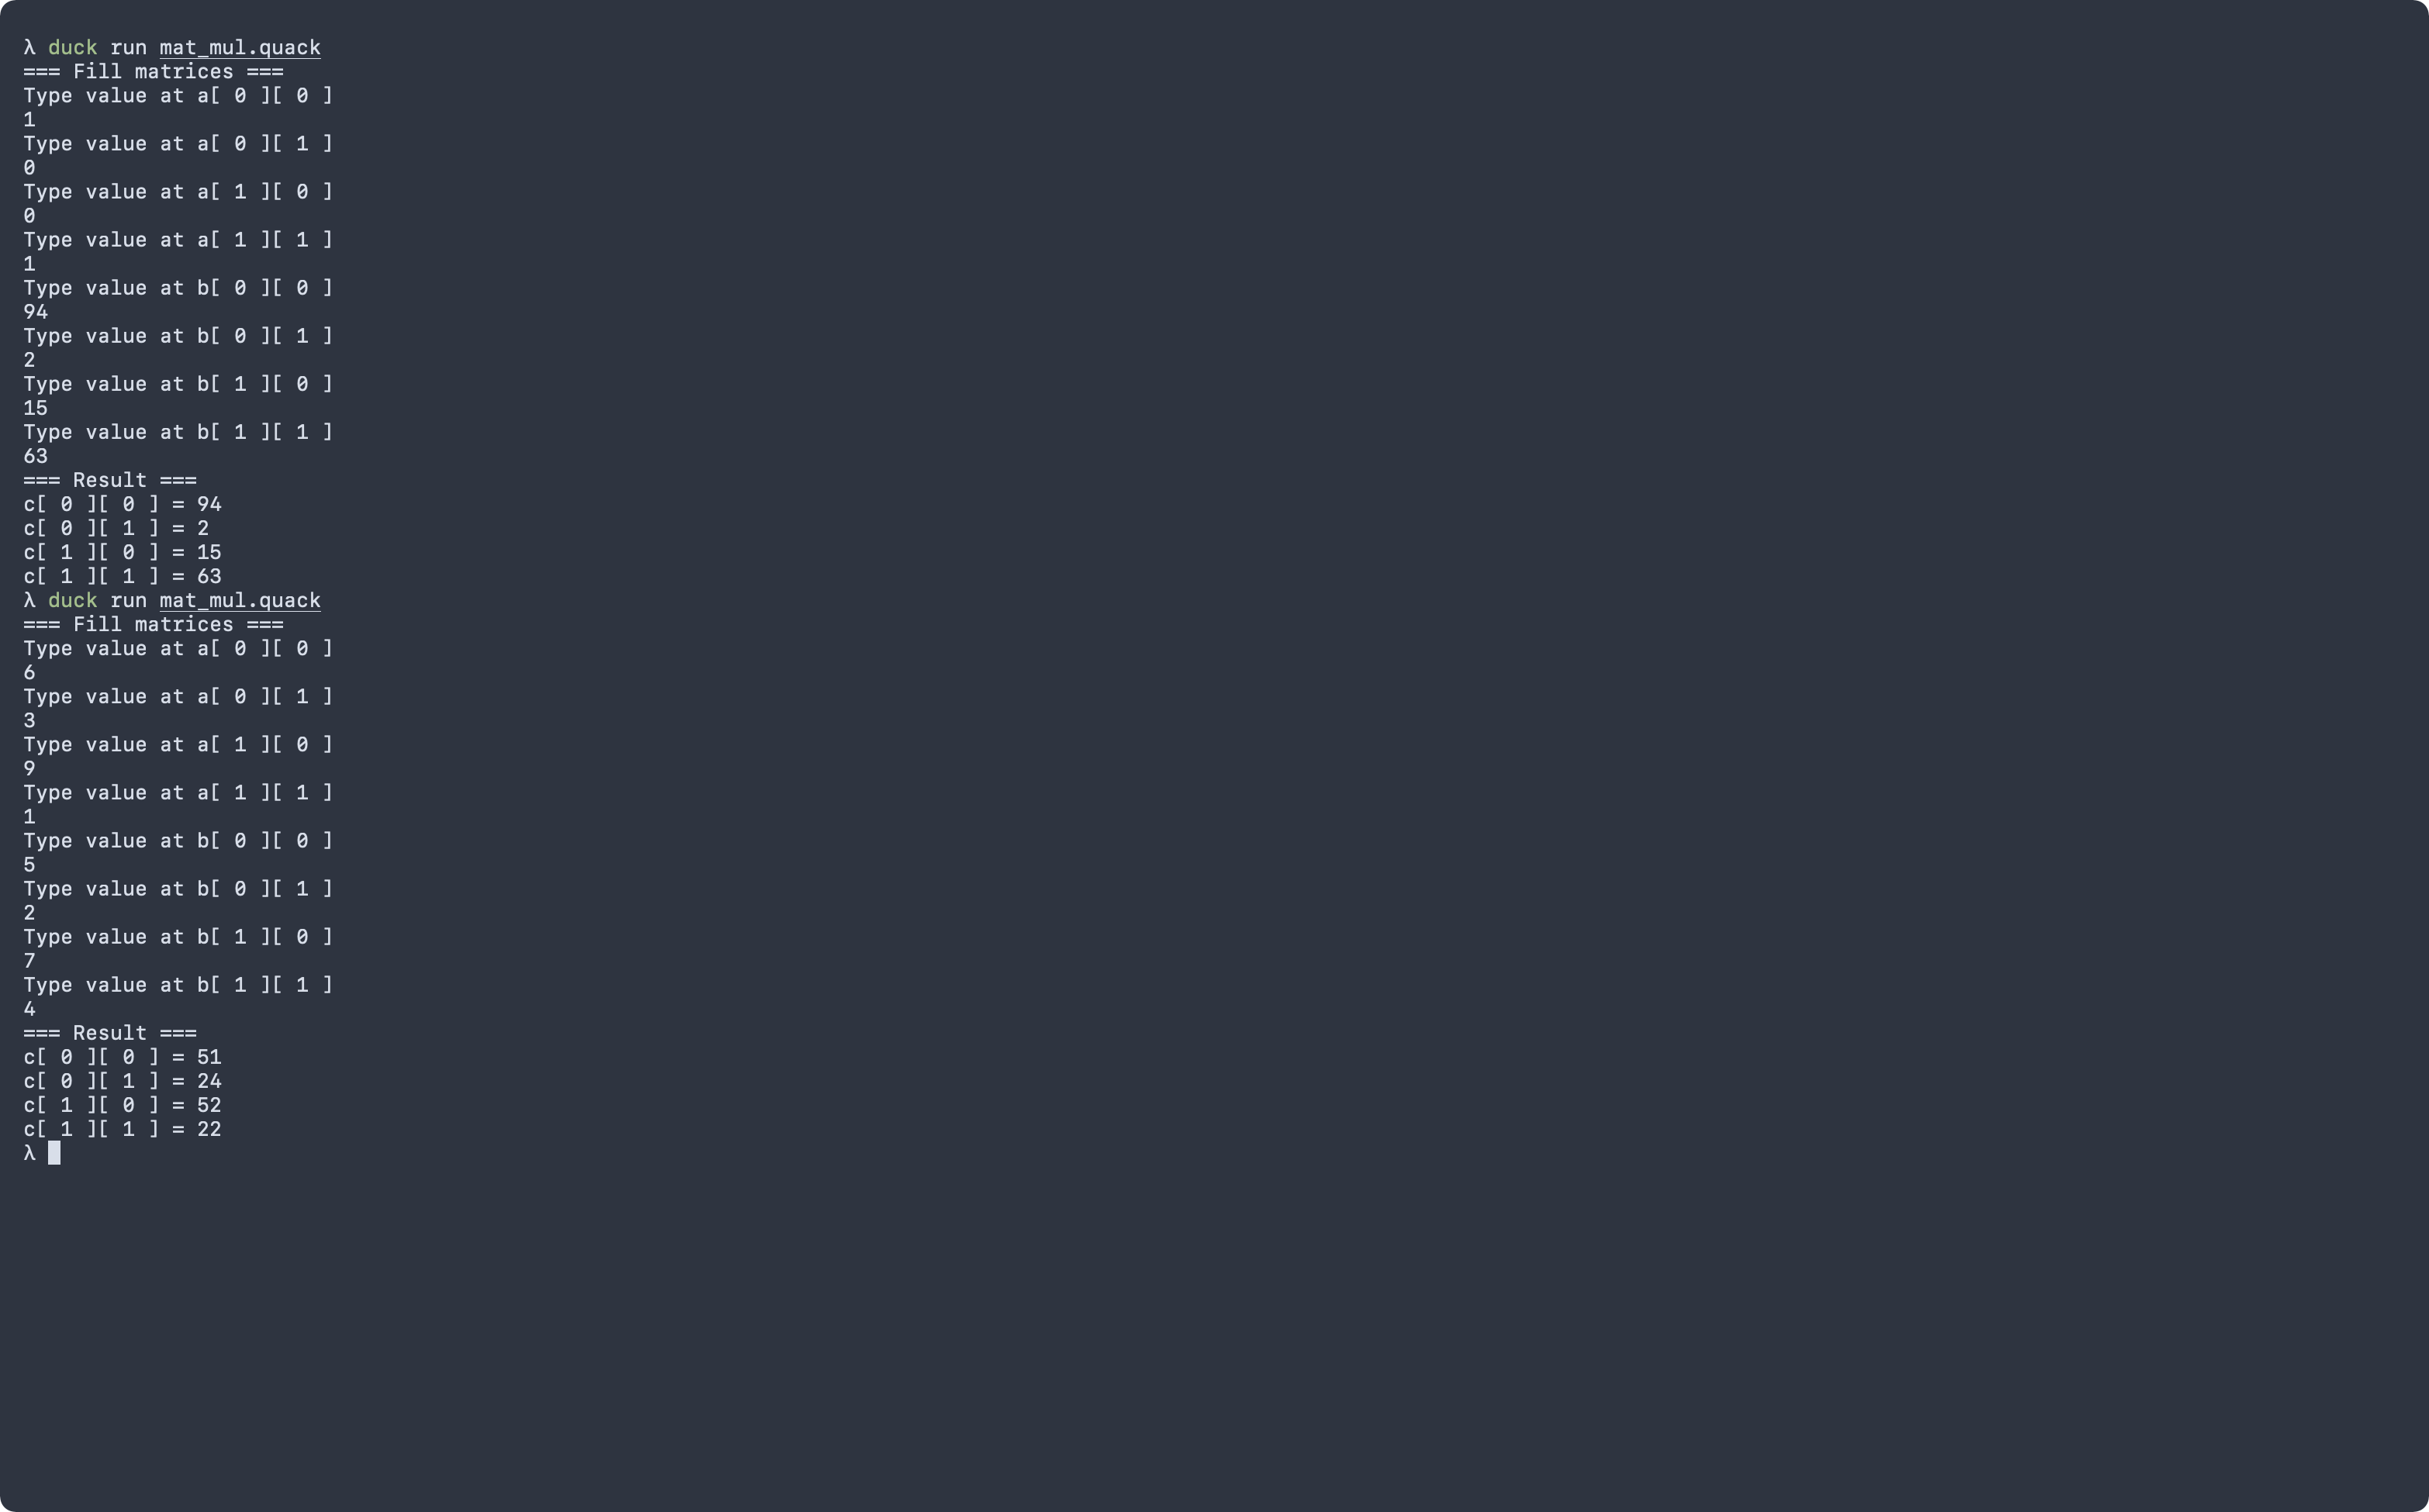
\includegraphics[width=\textwidth]{evidences/mat_mul_output}
\end{figure}

\newpage

\subsection{Built-in procedures}

\begin{verbatim}
proc main()
    var data [5]float;
    var pi, ans1, ans2, ans3 float;
{
    pi <- 3.14159;

    print("=== Trigonometric functions ===");

    ans1 <- sin(pi / 2);
    ans2 <- asin(ans1);
    print("sin(pi / 2) =", ans1, "asin(sin(pi / 2) =", ans2);

    ans1 <- cos(0);
    ans2 <- acos(ans1);
    print("cos(0) =", ans1, "acos(cos(0) =", ans2);

    ans1 <- tan(pi / 4);
    ans2 <- atan(ans1);
    ans3 <- atan2(1, 1);
    print("tan(pi /4) =", ans1);
    print("atan(tan(pi /4)) =", ans2, "atan2(1, 1) =", ans3);

    print("");
    print("=== Trascendental functions ===");

    ans1 <- exp(1);
    print(ans1);

    ans1 <- ln(ans1);
    print("ln(exp(1) =", ans1);

    ans1 <- log(125, 5);
    print("log(125, 5) =", ans1);

    print("");
    print("=== Other functions ===");

    ans1 <- pow(3, 5);
    print("pow(3, 5) =", ans1);

    ans1 <- sqrt(2);
    print("sqrt(2) =", ans1);

    ans1 <- mod(41, 3);
    print("mod(41, 3) =", ans1);

    ans1 <- abs(-12);
    print("abs(-12) =", ans1);

    ans1 <- ceil(1.5);
    print("ceil(1.5) =", ans1);

    ans1 <- floor(1.5);
    print("floor(1.5) =", ans1);

    print("");
    print("=== Vectorial functions ===");

    data[0] <- pi;
    data[1] <- exp(1);
    data[2] <- sqrt(2);
    data[3] <- (1 + sqrt(5)) / 2;
    data[4] <- 2;

    print("vector = [", data, "]");

    ans1 <- mean(data);
    ans2 <- median(data);
    ans3 <- mode(data);

    print("mean =", ans1);
    print("median =", ans2);
    print("mode =", ans3);
}
\end{verbatim}

\begin{figure}[H]
    \centering
    \caption{Generated IR code}
    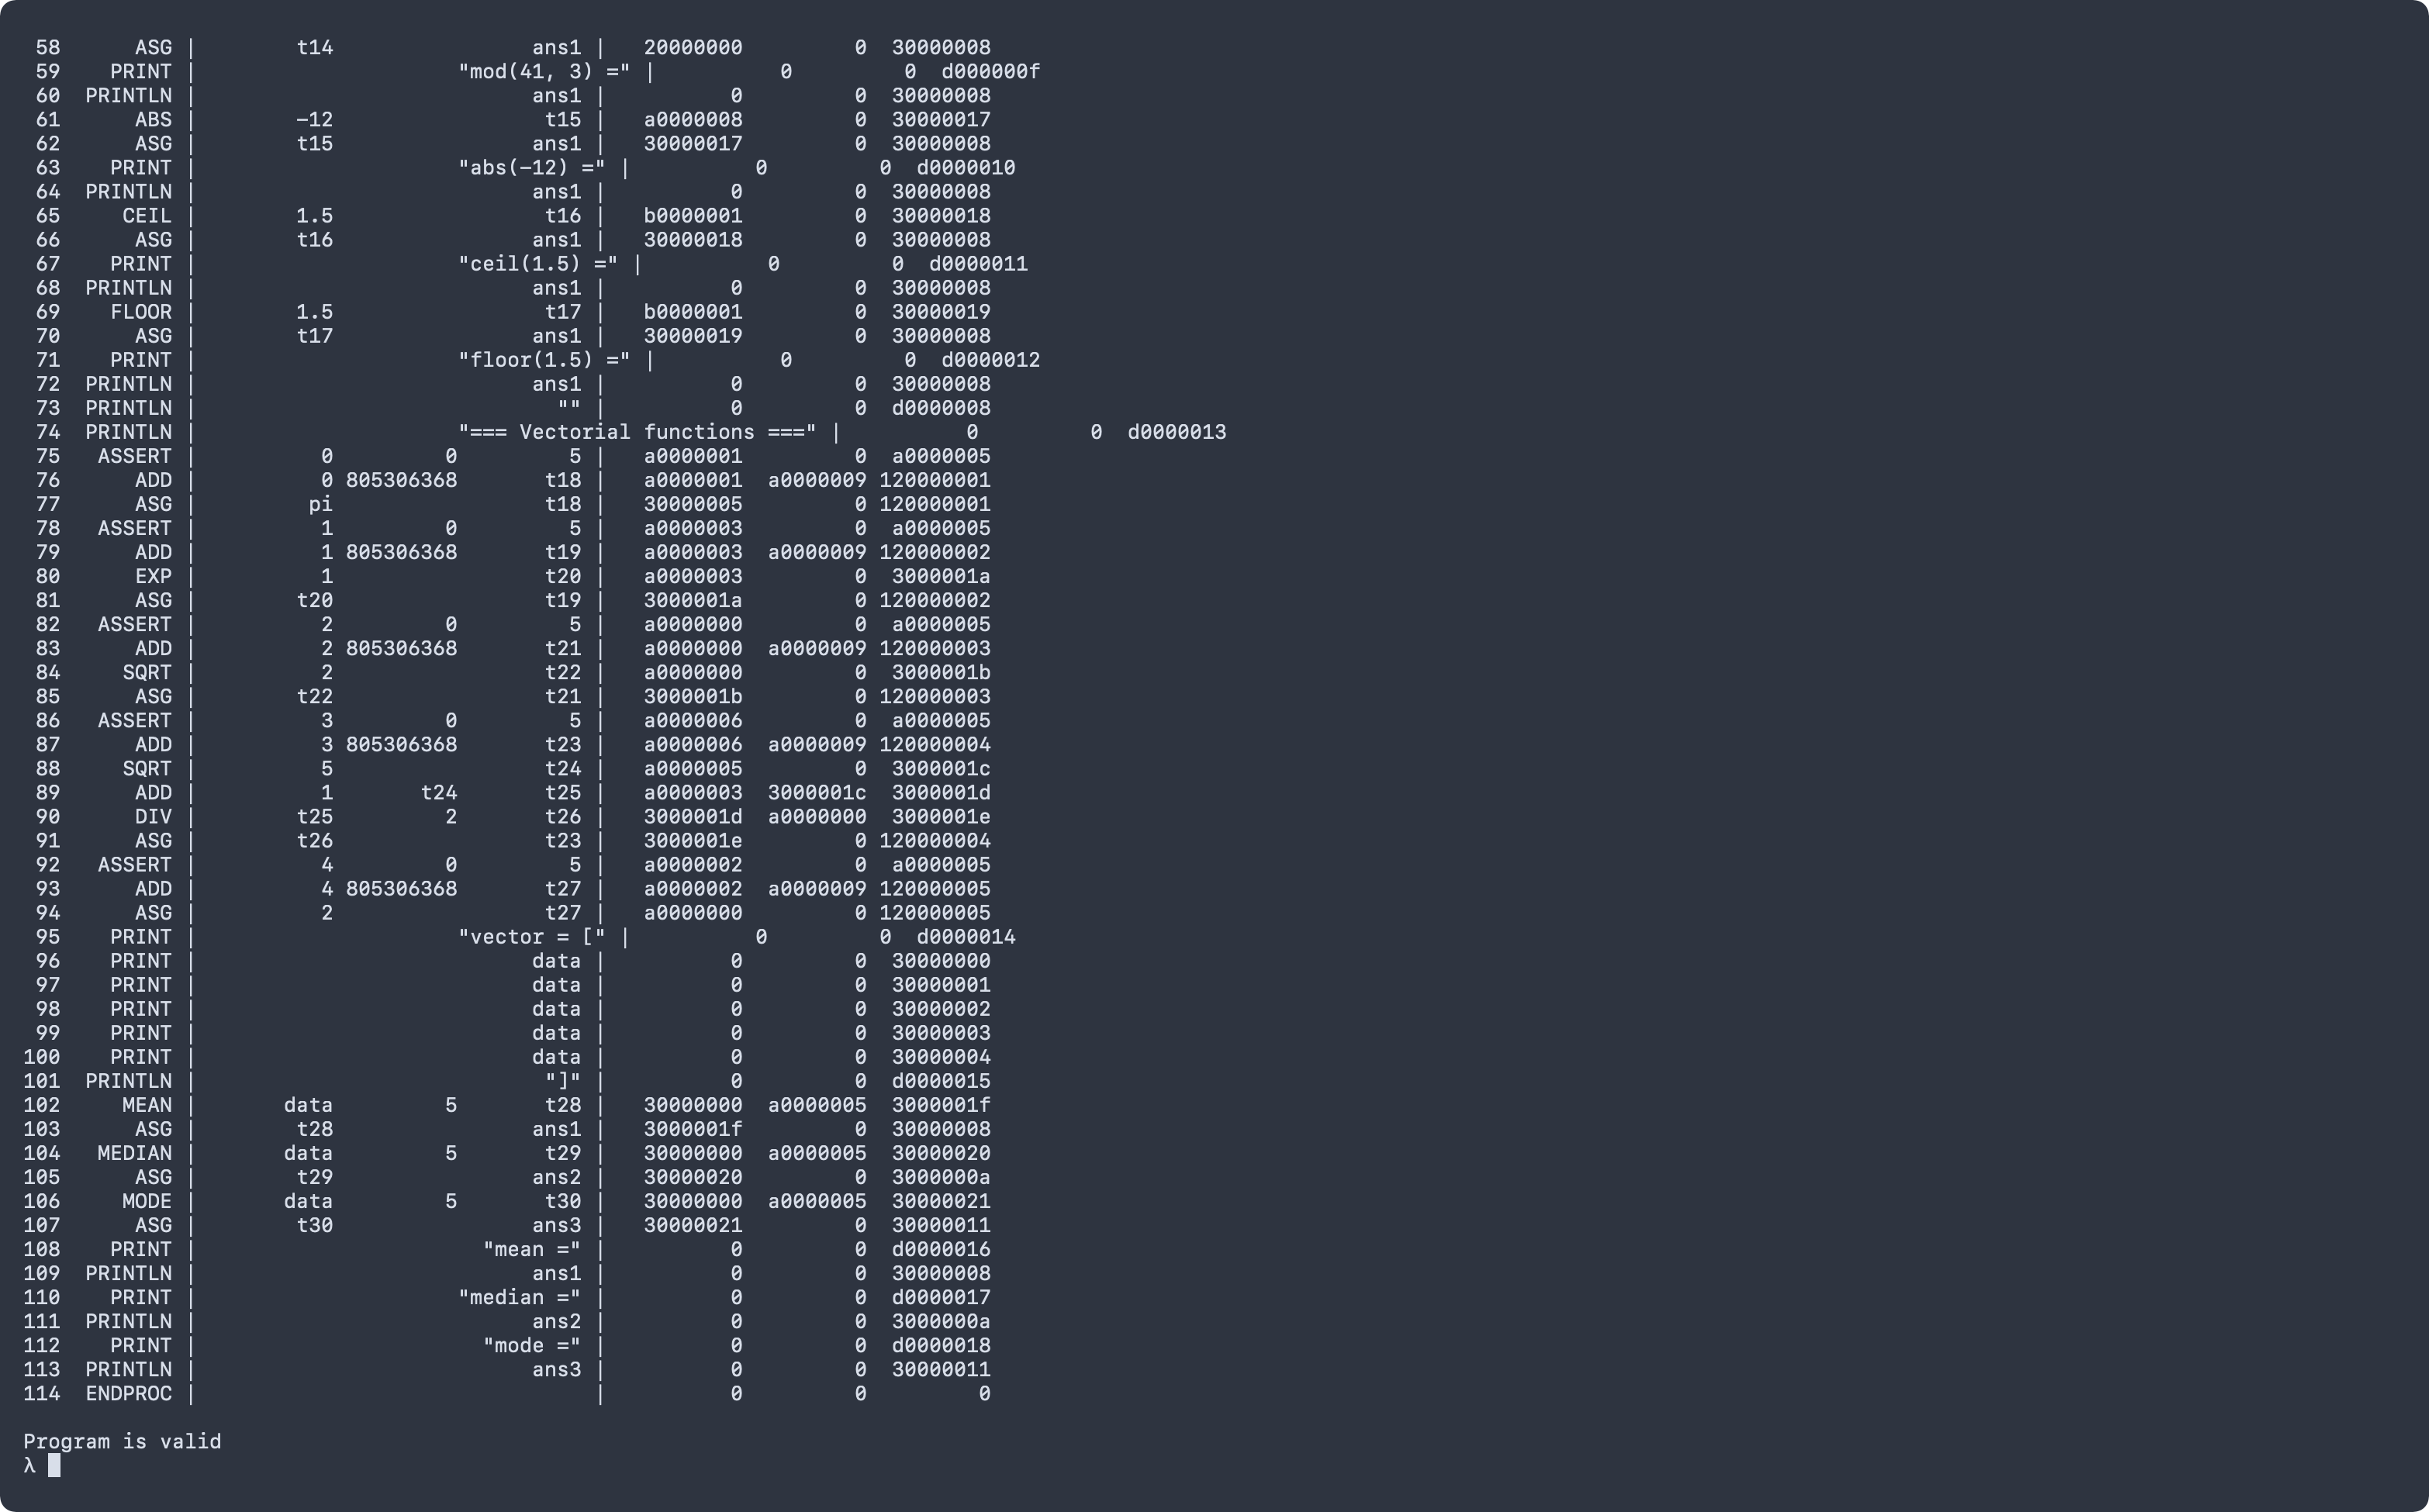
\includegraphics[width=\textwidth]{evidences/built_in_ir}
\end{figure}

\begin{figure}[H]
    \centering
    \caption{Program output}
    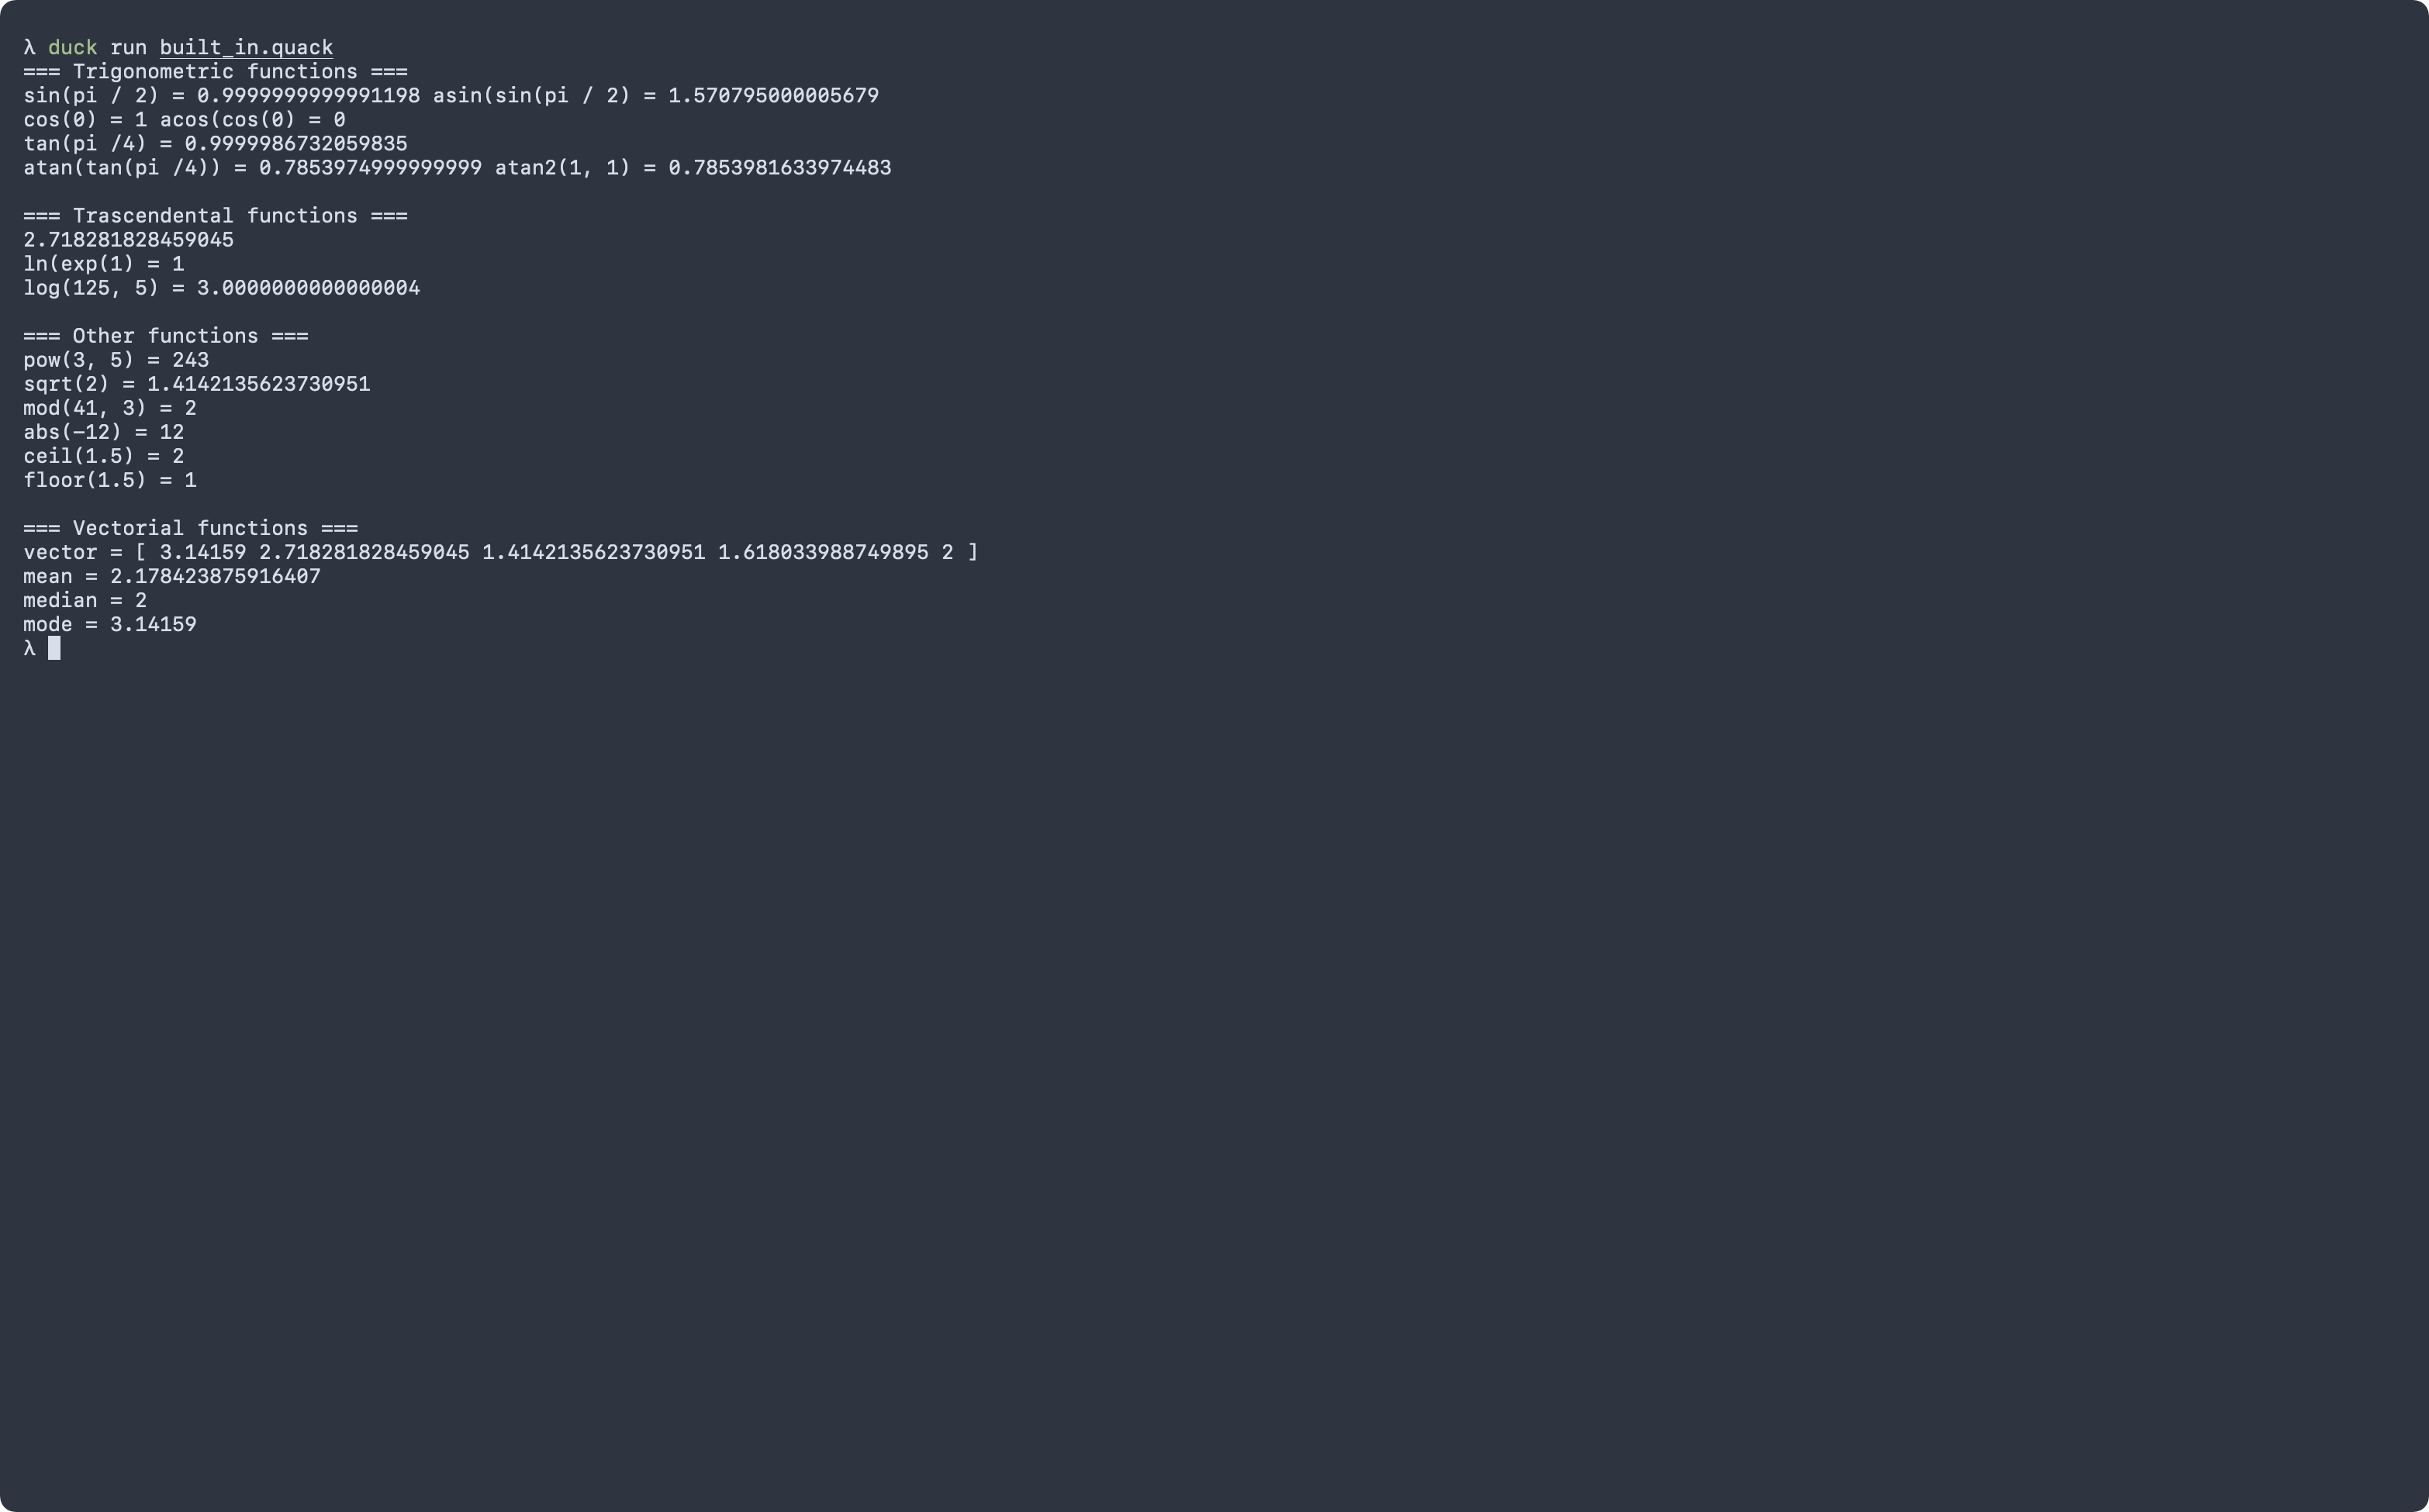
\includegraphics[width=\textwidth]{evidences/built_in_output}
\end{figure}

\newpage
